\documentclass[sigplan,10pt,nonacm,anonymous]{acmart}
\renewcommand\footnotetextcopyrightpermission[1]{}
\settopmatter{printfolios=true,printccs=false,printacmref=false}
\microtypesetup{expansion=false,protrusion=false}
\setcopyright{none}

\usepackage{amsmath,amssymb}
\usepackage{graphicx}
\usepackage{booktabs}
\usepackage{multirow}
\usepackage{xspace}
\usepackage{placeins}
\usepackage{algorithm}
\usepackage{algpseudocode}
\usepackage{xcolor}
\usepackage{enumitem}
\usepackage{fancyvrb}
\usepackage[switch]{lineno}
\renewcommand\linenumberfont{\normalfont\tiny\color{red!70!black}}
\sloppy
\emergencystretch=2em

\newcommand{\tool}{\textsc{ACC-Search}\xspace}
\newcommand{\todo}[1]{\textcolor{red}{[#1]}}

\citestyle{acmnumeric}

\begin{document}

\title{Composing Collectives Above a Black-Box Vendor Library:
A Closed-Stack Search Loop}
\author{Anonymous Authors}
\affiliation{%
  \institution{University of California, Berkeley}
  \city{Berkeley}\state{CA}\country{USA}
}
\email{anonymous@review.org}
\renewcommand{\shortauthors}{Anonymous}
\makeatletter
\AtBeginDocument{%
  \gdef\@author{Anonymous Authors}%
  \gdef\authors{Anonymous Authors}%
  \gdef\addresses{\@author{Anonymous Authors}}%
}
\makeatother

\begin{abstract}
Picking the fastest collective-communication strategy for a
distributed-training workload is hard. Timing each strategy on
a microbenchmark is cheap but can pick a strategy that is slow or
fails to compile inside a real training step. Running each
strategy end-to-end is direct, but realistic GPU-cluster
experiments are expensive. Cost-model simulators have been
explored, but existing ones are tuned against a fixed reference,
so their internal numbers drift across machines, model shapes,
and library versions. The simulator approach is even harder on
closed-source vendor stacks (AWS Trainium, Google TPU, Meta
MTIA), because of two specific properties: \emph{(C1) no
visibility into the runtime} --- when an operation is slow the
user cannot inspect the vendor library to see why --- and
\emph{(C2) no low-level control} --- vendor primitives are
called through a fixed API, with no exposed schedule-level
intermediate representation (which would let a user choose how
chunks are split, routed, or fused inside a collective).

This paper introduces a new design that addresses each of these
challenges. For (C1), we have an LLM agent build the cost-model
simulator on the target deployment itself: it writes probing
code that measures the simulator's internal numbers against the
actual device, model, and library version, so the simulator's
estimates re-adapt to the deployment whenever any of those
changes. For (C2), we accept the API as fixed and search one
layer above it: which primitives to call, in what order, and
how to reshape, pad, or slice the input/output tensors around
each call. Against an internal-AWS-optimized baseline used in
production on Trainium today, the deployed strategies deliver
\textbf{1.40$\times$} end-to-end speedup on OLMoE-10B at actual
training runs, with matched descent on real OpenWebText
(Figure~\ref{fig:loss-curve}), and \textbf{3.24$\times$} on
Llama-7B.
\end{abstract}

\pagestyle{plain}
\maketitle
\linenumbers
\modulolinenumbers[1]

\section{Introduction}
\label{sec:intro}

Choosing the fastest collective-communication strategy for a
distributed-training workload is challenging, and
two prevailing methods have substantial limitations. Running each
candidate strategy end-to-end on the actual workload is direct
but costly: realistic GPU-cluster experiments are expensive,
and the cost grows with the number of strategies tried.
Ranking strategies by a cheap microbenchmark on small
isolated calls is much cheaper, but on a Trainium cluster we
show that multiple strategies that win microbenchmarks are
materially \emph{slower} at actual training runs than a
different strategy that loses in microbenchmarks
(Figure~\ref{fig:disagree}). We call this \emph{cross-scope
inversion}: moving an operation from an isolated microbenchmark
into a real multi-rank training step changes the per-call cost,
because the surrounding training graph changes how the runtime
launches, fuses, and lays out tensors for the call.

A third approach, scoring strategies against a cost-model
simulator, has been explored in prior work
(SimAI~\cite{wang2025simai},
ASTRA-sim~\cite{rashidi2020astrasim,won2023astrasim2}). But
existing simulators are written and tuned against a fixed
reference configuration: the numbers they use internally ---
per-collective bandwidth, the overhead each time the runtime
launches a graph, when adjacent calls fuse, etc. --- drift
across machines, model shapes, and library versions,
and re-tuning them by hand for each new environment
or training task is again costly. The
simulator-based approach gets even harder on the closed-source
vendor stacks production training increasingly runs on (AWS
Trainium, Google TPU, Meta MTIA), because of two specific
properties of these stacks.
\textbf{(C1) No visibility into the runtime:} when an operation
(e.g., \texttt{xm.all\_to\_all} from Trainium) is unexpectedly slow, developers
cannot inspect the vendor library to see why --- its internals are
not source-available, and there are limited per-primitive 
configuration parameters to calibrate a simulator against.
\textbf{(C2) No low-level control:} the vendor's collective
primitives (\texttt{xm.all\_gather}, \texttt{xm.all\_to\_all},
\dots) are called through a fixed API; there is no exposed
schedule-level intermediate representation
--- which, in the open-stack systems
MSCCL~\cite{cowan2022msccl} and
TACCL~\cite{shah2023taccl} target, is the surface that lets a
user choose how chunks are split, routed through the network,
or fused inside a collective.

This paper introduces a new design that addresses each of
these challenges.
\textbf{For (C1)}, we approximate visibility into the closed
runtime by having an LLM agent build a cost-model simulator
on the target deployment itself: the LLM writes probing code
that measures the simulator's internal numbers against the
actual device, model shapes, and library version the workload
will use. This does not require internal visibility into the
runtime, but it gives a usable proxy for ``is this strategy
fast for this specific task?'' whose estimates re-adapt to the
deployment when any of the device, model, or library changes
--- so the simulator stays workload-faithful where a
hand-coded one would drift.
\textbf{For (C2)}, we do not try to recover low-level control.
We accept the vendor API as fixed and search one layer above
it --- over which primitives to call, in what order, and how
to reshape, pad, or slice the input/output tensors around each
call. The LLM proposes strategies at this layer; the
workload-calibrated simulator scores them; top-scoring
strategies are validated on real hardware before deployment.

One might ask: if the simulator's own internal numbers come
from on-device probes, isn't this just the microbenchmark
option in a different wrapper? Our ablation
(\S\ref{sec:ablation-nosim}) is set up to answer exactly that.
The difference is in \emph{what} we probe and \emph{how} we
probe it. Our simulator encodes hardware-specific performance
models, and the LLM is guided to calibrate them using probe
workloads that resemble real model-training settings (real
tensor shapes, full step boundaries, multi-rank dispatch
patterns), rather than the small isolated calls a standalone
microbenchmark would measure. The probes therefore capture
behavior that small microbenchmarks miss, while remaining far
cheaper than running a full training harness end-to-end on
each candidate strategy. When we ablate the simulator and let
the LLM rank strategies by its own small microbenchmarks
instead, the $1.40\times$ OLMoE-10B speedup collapses to
$1.00\times$: the LLM converges to structurally the same
strategy practitioners already deploy, because microbench
rankings are exactly what selected that strategy in the first
place. In other words, the work-load-faithful simulator, not
the LLM, is what picks the strategy that wins at actual
training runs.


\paragraph{Closed-stack collective communication library} A growing class of
production training accelerators operates on proprietary collective communication libraries. AWS Trainium~\cite{aws_trainium_neuron,
aws_trainium2_2024} --- 30--40\% better
price-performance than NVIDIA H100 on transformer workloads and
adopted at scale for Mixture-of-Expert (MoE) and Llama training --- ships a Neuron
Runtime that exposes collectives only through the PyTorch/XLA
integration (XLA = Accelerated Linear Algebra, PyTorch's
compiler bridge to non-NVIDIA accelerators) --- i.e.\ as
\texttt{xm.*} entry points such as
\texttt{xm.\allowbreak{}all\_gather} --- behind which the Neuron
compiler emits NEFF binaries (Neuron Executable File Format;
the compiled artifact loaded onto each NeuronCore) from
unpublished sources. There is no
user-configurable schedule layer: per-collective chunking and
network-interface-card (NIC) routing cannot be reached from
above the runtime. Google TPU and Meta MTIA exhibit the same
constraint: the programmable schedule surface that MSCCL- and
TACCL-style synthesis depend on is not exposed. The schedule-synthesis paradigm
of the open-stack era cannot be ported here in any straightforward
way. Above the \texttt{xm.*} (or equivalent vendor) boundary, the
design choice that remains is which primitive to call, in what
order, and against what tensor layout. We refer to this as the \emph{strategy} layer,
in contrast to the \emph{schedule} layer that MSCCL/TACCL
operate on, which decides how each collective message is split
into chunks, which network paths each chunk takes, and how the
chunks are pipelined across devices. The strategy layer is less expressive
but, as we show, contains strategies $1.4$--$3.2\times$ faster
than the developer baseline.

\paragraph{Related schedule-synthesis work and why it does not
apply here.} Automated synthesis of collective-communication
algorithms has been studied at the \emph{schedule} layer ---
which message chunks move along which paths, in what order, against
which network adapters. MSCCL and MSCCLang~\cite{cowan2022msccl}
emit XML or DSL schedules for the NCCL/RCCL runtime~\cite{nvidia_nccl} to consume;
TACCL~\cite{shah2023taccl} uses a sketch language and an SMT
solver; AutoCCL~\cite{xu2025autoccl} adds tuning;
SCCL~\cite{cai2021sccl} synthesizes Pareto-optimal algorithms
from first principles. All share an infrastructural prerequisite:
the underlying runtime exposes a programmable intermediate
representation (IR) for the schedule.


\paragraph{Validation and contributions.}
We validate our design on the eight collective problems listed
in Table~\ref{tab:problems} --- four that arise in
Mixture-of-Expert (MoE) training~\cite{shazeer2017outrageously}
and four that arise in dense-transformer (Llama-style) training
--- on a 7-node \texttt{trn1.32xlarge} cluster (224 ranks).

\begin{table}[h]
\centering\scriptsize
\setlength{\tabcolsep}{3pt}
\setlength{\abovecaptionskip}{2pt}
\setlength{\belowcaptionskip}{-2pt}
\begin{tabular}{@{}p{0.28\columnwidth}p{0.67\columnwidth}@{}}
\toprule
\textbf{Problem} & \textbf{Role in the training step} \\
\midrule
\multicolumn{2}{@{}l}{\textit{MoE-side}} \\
AllToAllV~\cite{lepikhin2021gshard}      & MoE token dispatch/combine; counts vary \\
Uniform AllToAll~\cite{zhou2022expertchoice} & MoE dispatch/combine; counts equal \\
Ring KV~\cite{liu2024ringattention}      & rotate KV shards around the rank ring \\
Distributed CE~\cite{shoeybi2019megatron} & loss over rank-sharded vocabulary \\
\midrule
\multicolumn{2}{@{}l}{\textit{Llama-side}} \\
PP cross-stage~\cite{huang2019gpipe}     & activations/grads between PP stages \\
TP MLP~\cite{shoeybi2019megatron}        & all-reduce after MLP in tensor parallel \\
FSDP weight prefetch~\cite{zhao2023pytorchfsdp} & gather sharded weights per layer \\
Layer-block AR~\cite{korthikanti2023reducing} & all-reduce grads at layer blocks \\
\bottomrule
\end{tabular}
\caption{The eight collective problems we evaluate.}
\label{tab:problems}
\end{table} The baseline we measure against is the
\emph{internal-AWS-optimized strategy} AWS uses in production
today to train large-scale MoE and dense transformer models on
Trainium, built and maintained by five experienced AWS
developers. On OLMoE-10B the deployed agent strategy delivers
\textbf{1.40$\times$} steady-state step-time speedup with
matched descent on a 2500-step
real-OpenWebText~\cite{Gokaslan2019OpenWeb} AdamW run
(Figure~\ref{fig:loss-curve}); on Llama-7B it delivers
\textbf{3.24$\times$}. Per-primitive per-step speedups range
$4$--$12\times$, above the end-to-end ratio because constant
non-collective compute dilutes the headline.

The contributions are
(i)~to our knowledge the first system that finds faster
collective-communication strategies on top of a closed-source
vendor library, delivering \textbf{1.40$\times$} end-to-end on
OLMoE-10B and \textbf{3.24$\times$} on Llama-7B over the
production baseline;
(ii)~a cost-model simulator whose per-term constants are
re-fit per-environment by LLM-written on-device probes,
keeping the simulator workload-faithful without
hand-coding new probe scripts for each cluster; and
(iii)~the closed-stack search loop combining the above with
LLM-driven mutation and hardware validation, with code
emitted as drop-in runtime modules and algorithm-equivalent
descent verified on real tokens.

\paragraph{Scope and generalization.} We instantiate our design
on AWS Trainium. The six cost-model terms are Trainium-specific,
but the categories they fall into (per-graph-launch overhead,
per-collective bandwidth ceiling, device-vs.-host copy cost,
runtime cache-reload cost) are general to closed-source vendor
runtimes that compile their own collective binaries. Google TPU
and Meta MTIA each expose closed equivalents; we expect the
strategy-search design to port with the cost-model term set
re-calibrated, and leave that to follow-up work.

\section{Related Work}
\label{sec:related}

\paragraph{Distributed training systems above the collective layer.}
Systems such as ZeRO~\cite{rajbhandari2020zero, ren2021zerooffload},
DeepSpeed~\cite{rasley2020deepspeed},
Megatron-LM~\cite{shoeybi2019megatron, korthikanti2023reducing,
narayanan2021efficient}, PyTorch DDP and
FSDP~\cite{li2020pytorch, zhao2023pytorchfsdp},
GPipe~\cite{huang2019gpipe}, PipeDream~\cite{narayanan2019pipedream},
Horovod~\cite{sergeev2018horovod}, BytePS~\cite{jiang2020byteps}, and
FlexFlow~\cite{jia2019flexflow} optimize a different layer than
this paper does: they decide \emph{how the training job itself is
laid out across devices} --- how model weights, optimizer states,
activations, and microbatches are partitioned, replicated, or
pipelined --- and then leave the collective calls themselves to
the underlying runtime (NVIDIA's collective-communication library
NCCL~\cite{nvidia_nccl} or AMD's equivalent RCCL on open stacks,
or to a schedule-synthesis framework like
MSCCL~\cite{cowan2022msccl} or TACCL~\cite{shah2023taccl} where
that is available). Our search instead fixes the model-parallel
layout and optimizes the next layer down: \emph{how each
individual collective is implemented} --- which vendor primitive
to call, in what order, and how to reshape, pad, or slice the
input/output tensors around each call --- against the closed
Trainium API where \texttt{xm.*} primitives cannot be modified or
introspected. Strategy-layer systems do not catch
vendor-specific pathologies on this stack (e.g.,
\texttt{xm.all\_to\_all} fails to compile across multiple nodes
on Trainium; a tensor reshape that looks free on paper actually
forces the runtime to physically copy the full tensor at slower,
non-sequential memory bandwidth), and schedule-synthesis
frameworks rely on rewriting schedules \emph{below} the runtime
boundary, which Neuron disallows. We treat \texttt{xm.*} as
fixed and search strategies \emph{above} it.

\paragraph{Cost-model simulators for distributed training.}
SimAI~\cite{wang2025simai},
ASTRA-sim~\cite{rashidi2020astrasim}, and
ASTRA-sim~2.0~\cite{won2023astrasim2} score training-system
choices against a cost-model simulator instead of running them
end-to-end. They are written and tuned against a fixed reference
configuration; we discuss the resulting drift problem and our
LLM-recalibrated alternative in \S\ref{sec:intro} and
\S\ref{sec:cost}.

\paragraph{Collective synthesis below an open boundary.}
A line of work synthesizes collective algorithms by exposing the
in-fabric schedule: SCCL~\cite{cai2021sccl} casts it as a constraint
problem; MSCCL/MSCCLang~\cite{cowan2022msccl} compiles a DSL to an
NCCL schedule IR; TACCL~\cite{shah2023taccl} adds communication
sketches and topology-aware search; Blink~\cite{wang2023blink}
targets multi-GPU servers; CoCoNet~\cite{jangda2022breaking}
jointly optimizes compute+communication;
AutoCCL~\cite{xu2025autoccl} auto-tunes low-level NCCL parameters
under compute-comm interference. All depend on a vendor library
that allows replacing or parameterizing the in-fabric schedule, a
prerequisite met on open NVIDIA/AMD stacks but not on closed-stack
accelerators such as AWS Trainium (Neuron Runtime), Google TPU
(where collectives are emitted by the XLA compiler as nodes in
its compute-graph IR, called HLO --- High-Level Operations), and
Meta MTIA --- where the in-fabric schedule lives behind a vendor
compiler and is not externally addressable. The Neuron stack we use as our case study
has no analogue of MSCCL-IR; we therefore search above the
primitives, not beneath them. The same closed-stack constraint
holds on TPU and MTIA, which makes the strategy-search
paradigm we describe potentially applicable to them as well
(§\ref{sec:future}).

\paragraph{Algorithm discovery with LLMs.}
FunSearch~\cite{romera2024funsearch} pioneered the LLM-as-mutator
loop for mathematical discovery;
AlphaEvolve~\cite{novikov2025alphaevolve} extended it to
code-level optimization;
ShinkaEvolve~\cite{lange2025shinkaevolve} emphasized
sample-efficient open-ended evolution.
AlphaTensor~\cite{fawzi2022alphatensor} and
AlphaDev~\cite{mankowitz2023alphadev} use deep RL for
matmul/sorting discovery. LLM code-generation work
(Codex~\cite{chen2021codex}, AlphaCode~\cite{li2022alphacode},
Self-Refine~\cite{madaan2023selfrefine},
Reflexion~\cite{shinn2023reflexion},
ToT~\cite{yao2023tot},
Self-Instruct~\cite{wang2023selfinstruct}) further established
LLMs as practical mutation oracles given a feedback loop. All
search the \emph{algorithm} or \emph{program text} space; in our
setting the same strategy admits many syntactic forms and the
cost surface is dominated by hardware quirks (NEFF cache, EFA
pipelining, implicit copies) none of these frameworks model. We
take the LLM-mutation loop structure from this lineage and graft
it onto a closed-stack-appropriate cost function; the headline
configuration is a single-trajectory ReAct agent because in our
setting the cost model and profiling toolkit already do the work
island parallelism would otherwise do — and the single-trajectory
variant is cheaper. Multi-island appears as an ablation.

\paragraph{Kernel autotuning and graph optimization.}
TVM~\cite{chen2018tvm}, AutoTVM~\cite{chen2018autotvm},
Ansor~\cite{zheng2020ansor} search kernel-implementation choices;
Halide~\cite{ragankelley2013halide} and
Triton~\cite{tillet2019triton} provide DSLs;
Tensor Comprehensions~\cite{vasilache2018tc},
MLIR~\cite{lattner2021mlir}, TASO~\cite{jia2019taso} operate at
the graph level. LLM-driven kernel-optimization systems
(STARK~\cite{stark2025}, K-Search~\cite{ksearch2026},
Astra~\cite{astra2025}, KernelEvolve~\cite{kernelevolve2025})
refine individual GPU kernels by 1.25--17$\times$. Our problem
is one level above: the Neuron compiler writes each
\texttt{xm.*} kernel; we vary which primitives are composed and
how, not their internal schedule.

\paragraph{MoE and Llama communication patterns.}
The Sparsely-Gated MoE
layer~\cite{shazeer2017outrageously},
GShard~\cite{lepikhin2021gshard},
Switch~\cite{fedus2022switch}, ST-MoE~\cite{zoph2022stmoe},
DeepSpeed-MoE~\cite{rajbhandari2022dsmoe},
Mixtral~\cite{jiang2024mixtral},
DeepSeekMoE~\cite{dai2024deepseekmoe}, and
OLMoE~\cite{muennighoff2024olmoe} together established that MoE
expert dispatch dominates the training step once active parameters
exceed a few hundred million. Expert-choice
routing~\cite{zhou2022expertchoice} fixes per-expert receive
counts and removes per-step host-side count computation from the
AllToAllV path; we use it in the end-to-end OLMoE evaluation.
On Llama~\cite{touvron2023llama, touvron2023llama2}, the PP
cross-stage send/recv $+$ TP MLP $+$ FSDP weight-prefetch
strategy we evaluate matches the standard training recipe.
Trainium practitioners typically issue one collective per
microbatch (e.g.\ one TP-MLP all-reduce per microbatch for a
training step of $M$ microbatches uses $M$ all-reduce calls).
We show that, when the per-microbatch payloads can share an
underlying buffer, the same logical strategy can also be
implemented by issuing a single collective per training step
that covers all $M$ microbatches at once --- trading $M$
launch costs for one. Whether this trade is profitable depends
on the device (a larger payload may take longer to compile or
exceed memory limits), so we let the search make that choice
per problem rather than fixing it by hand.


\section{System Model}
\label{sec:model}

\subsection{The search loop}

\paragraph{Notation.} A collective problem $p$ has a pure-Python
reference $\mathrm{ref}_p(\cdot)$ encoding correctness; a seed
library $\mathcal{S}_p$ of human-written candidate strategies; and
fixed I/O shapes. The search space $\Sigma_p$ is the set of Python
functions with $p$'s signature that compose primitives from the
vendor set
\begin{equation*}
\begin{aligned}
\mathcal{V} \;=\; \{ &\texttt{all\_gather},\; \texttt{reduce\_scatter},\; \texttt{all\_reduce},\\
                     &\texttt{collective\_permute},\; \texttt{all\_to\_all} \,\}
\end{aligned}
\end{equation*}
(all in the \texttt{xm.*} family) together with local XLA ops. A candidate $s \in \Sigma_p$ is admissible if it
matches the reference,
\[
\textsc{Correct}(s) \;=\; \forall \textsc{ws} \in \{4, 8\}:
   \; s(\cdot) = \mathrm{ref}_p(\cdot).
\]
Phase~1 fits a Trainium cost model
$\mathrm{Sim}: \Sigma_p \to \mathbb{R}_{\ge 0}$ from on-device
measurements (Section~\ref{sec:cost}). Phase~4 applies a hardware test that runs the strategy on real
Trainium hardware at the training-shape configuration, returning
$\textsc{Gate}(s) \in \{0, 1\}$ for whether the strategy compiled
and ran without error.
The deployed strategy is
\begin{equation*}
\begin{aligned}
s^\star_p &\;=\; \arg\min_{s \in \Sigma_p^\dagger}\; \mathrm{Sim}(s), \\
\Sigma_p^\dagger &\;=\; \{s \in \Sigma_p : \textsc{Correct}(s) \wedge \textsc{Gate}(s)=1\}.
\end{aligned}
\end{equation*}
The LLM $\mathcal{M}$ acts as a stochastic proposer
$\mathcal{M}: \Sigma_p \to \Sigma_p$ that mutates candidates;
Phase~3 instantiates this as one of three search shapes
(strategy-enumerate / cc-react / multi-island) over a bounded
$\mathcal{M}$-call budget. The five sequential phases that
implement this loop are illustrated in
Figure~\ref{fig:workflow}.

\begin{figure}[t]
\centering
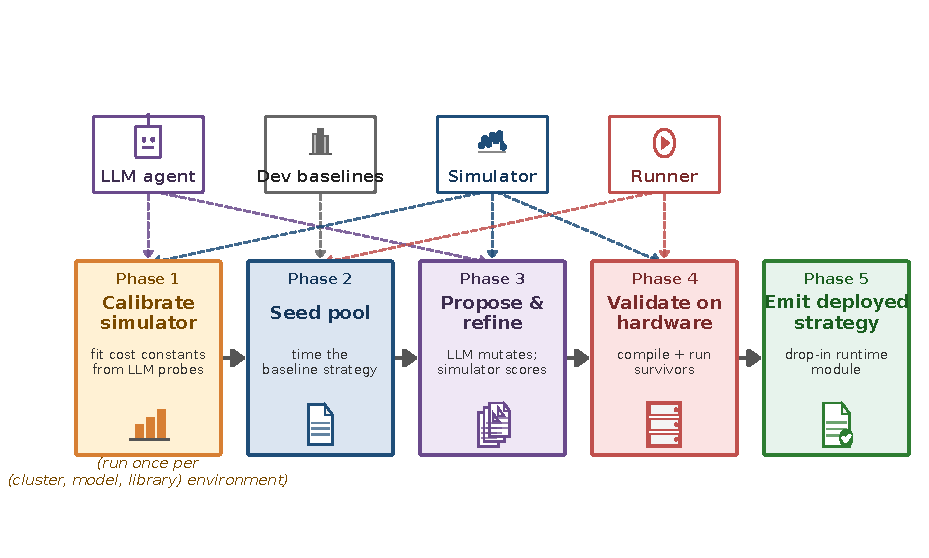
\includegraphics[width=0.95\linewidth]{figures/workflow.pdf}
\caption{Closed-stack search loop. The training workload
supplies tensor shapes and the primitive set. An LLM agent
plays two roles: it writes hardware-specific probing code that
calibrates a workload-faithful cost model on the target device,
and it proposes candidate strategies whose predicted step time
the cost model scores. The top-scoring candidate is validated on
real hardware before being emitted as a drop-in runtime
module. The rest of this section expands the loop into five
sequential phases.}
\label{fig:workflow}
\end{figure}

\paragraph{Phase~1: agent-driven on-device calibration.}
Throughout the paper we refer to the LLM-driven search loop as the
\emph{agent}: a process that proposes, scores, and refines
candidate strategies through several phases. In Phase~1, the
agent is given a set of measurement \emph{tools} (listed in
Table~\ref{tab:probe-tools}) and designs the probe campaign
autonomously: which tensor sizes to sweep, which primitives to
compare, how many repetitions to run, and when to test whether
a measured number really comes from the term it is meant to
isolate (e.g.\ rule out hidden memory-copy overhead by varying
whether the input tensor is stored contiguously in memory). Each tool returns
an empirical scalar or function that wires into one term of
Eq.~\ref{eq:cost}; the agent produces the numerical constants that
populate the simulator. We supply the tools (so the LLM cannot
fabricate numbers), not the experimental design (so the LLM
exploits domain knowledge to choose more informative probes than a
hardcoded script would). Two terms used in the tool list are
worth defining: \emph{EFA} (Elastic Fabric Adapter) is AWS's
RDMA-based cross-node network fabric, used by the cross-node
point-to-point probe; \emph{amortization}, in the back-to-back
tool, refers to the empirical observation that the cost of $k$
consecutive collective calls is typically less than $k$ times
the cost of one call, because the runtime can overlap some of
the per-call overhead across consecutive calls. The tool API
and sweep grids are in Appendix~\ref{sec:profile-impl}.

\begin{table}[!htbp]
\centering\footnotesize
\setlength{\tabcolsep}{3pt}
\setlength{\abovecaptionskip}{2pt}
\setlength{\belowcaptionskip}{0pt}
\begin{tabular}{ll}
\toprule
\textbf{Tool} & \textbf{What it measures} \\
\midrule
\texttt{m\_collective\_lat}   & per-prim latency vs.\ bytes / world size \\
\texttt{m\_p2p\_transfer}     & cross-node point-to-point bandwidth over EFA \\
\texttt{m\_xla\_op\_overhead} & per-op floors for local XLA ops \\
\texttt{m\_compilation\_cost} & cold / cache / reload NEFF compile times \\
\texttt{m\_launch\_overhead}  & per-graph-dispatch (\texttt{mark\_step}) tax \\
\texttt{m\_memcopy\_thru}     & seq.\ and strided host/device copy bw \\
\texttt{m\_b2b\_amortization} & amortization curve for $k$ consecutive collectives \\
\bottomrule
\end{tabular}
\caption{Phase-1 measurement tools the agent is given (prefix
\texttt{m\_} = \texttt{measure\_}). Full identifiers in
Appendix~\ref{sec:profile-impl}.}
\label{tab:probe-tools}
\end{table}

\paragraph{Phase~2: Baseline evaluation.}
A per-problem library of seeded templates is scored through the
simulator. The seed library always contains the
\emph{internal-AWS-optimized baseline} strategy for that
primitive plus a small number of workable but typically naive or
slower alternatives; the per-problem seed lists are given in
Appendix~\ref{sec:phase-code} as code boxes. The baseline we
measure against throughout the paper is the strategy AWS
\emph{uses in production today} to train large-scale MoE and dense
transformer models on Trainium. It is built and confirmed by five
experienced AWS developers who write and maintain Trainium
training paths professionally. The result is the optimized
strategy practitioners actually deploy, not a strawman. The LLM
is not told which seed is the baseline pick. This both calibrates
the simulator's ordering against established practice and seeds
Phase~3.

\paragraph{Phase~3: Agent-driven search.}
The search style we use is \textbf{strategy-enumerate}: the LLM
enumerates $K$ structurally distinct strategies as
natural-language sketches (``pack and gather'', ``per-source
slice loop'', ``masked all-reduce over stacked microbatches'',
$\ldots$), implements each independently, then refines the top-2
by simulator score under a bounded budget
(\S\ref{sec:strat-enum}).

\paragraph{Phase~4: Hardware validation.}
Each Phase-3 survivor runs through a 20-iteration hardware (HW)
microbench plus a 10-step training-validation (TV) harness on a
synthetic 8-layer LM. Crashes, OOMs, NaN at world-scale, or
shape-gate failures exclude the candidate regardless of simulator
score; failed candidates get LLM-assisted recovery (up to two
attempts). HW timing itself is not the ranking signal.

\paragraph{Phase~5: Code generation.}
The lowest \emph{simulator-score} survivor among HW$+$TV passers
wins. We do not pick by HW microbench directly because the
microbench measures isolated-call latency with cached NEFFs and
does not surface the NEFF cache-eviction cost that appears in
real training.

\begin{algorithm}[!htbp]
\caption{End-to-end closed-stack collective-strategy search.}
\label{alg:pipeline}
\begin{algorithmic}[1]
\Require $P$, $\mathrm{ref}(\cdot)$, $\mathcal{S}_P$,
LLM $\mathcal{M}$, profiling tools $\mathcal{T}$, hardware $H$.
\Ensure deployable \texttt{runtime/trainium\_<P>.py}.
\smallskip
\State $\Theta \gets \mathcal{M}.\textsc{calibrate}(\mathcal{T}, H)$
\Comment{Phase~1}
\State $\mathrm{Sim}(\cdot) \gets \textsc{BuildCost}(\Theta)$
\Comment{Eq.~\ref{eq:cost}}
\smallskip
\For{$s \in \mathcal{S}_P$}\Comment{Phase~2}
  \State $\mathrm{score}(s) \gets \mathrm{Sim}(s)$;
  $\textsc{Verify}(s, \mathrm{ref}, \textsc{ws}{\in}\{4,8\})$
  \Comment{verify on small rank counts $\textsc{ws}\!\in\!\{4,8\}$}
\EndFor
\smallskip
\State $\mathcal{C} \gets \textsc{InitPool}(\mathcal{S}_P)$
\Comment{Phase~3 (strategy-enumerate)}
\For{$r = 1 \ldots R$}
  \State $s' \gets \mathcal{M}.\textsc{propose}(\mathcal{C}, \Theta)$
  \If{$\neg\,\textsc{Verify}(s', \mathrm{ref})$} \textbf{continue} \EndIf
  \State $\mathrm{score}(s') \gets \mathrm{Sim}(s')$;
  $\mathcal{C} \gets \mathcal{C} \cup \{s'\}$.
\EndFor
\smallskip
\For{each Phase-3 survivor $s$}\Comment{Phase~4}
  \State $t_{\mathrm{hw}}(s) \gets \textsc{Microbench}(s, H)$
  \State $\textsc{ShapeGate}(s, H)$;
         $\textsc{TVGate}(s, H)$.
  \State $s \gets \mathcal{M}.\textsc{recover}(s)$ \textbf{if}
  gate fails (up to $2\times$).
\EndFor
\smallskip
\State $s^\star \gets \arg\min_{s \in \text{survived}}\,\mathrm{Sim}(s)$
\Comment{Phase~5}
\State $\textsc{Emit}(\texttt{runtime/trainium\_<P>.py},\, s^\star)$;
deploy to $H$.
\end{algorithmic}
\end{algorithm}

\subsection{Cost model}
\label{sec:cost}

The simulator builds a per-step time estimate as the sum of six
physically-grounded terms:
\begin{equation}
\label{eq:cost}
\begin{aligned}
T_{\text{step}} \;=\;
& \underbrace{\textstyle\sum_{i \in \mathcal{L}} c(\mathrm{op}_i, b_i)}_{T_{\text{local}}}
\;+\;
\underbrace{\textstyle\sum_{j} \max(d^{(j)}_{\text{amort}}, b_j / w_{\text{eff}})}_{T_{\text{bw}}} \\
& \;+\;
\underbrace{d_{\text{full}} + (k{-}1)\,d_{\text{amort}}}_{T_{\text{coll}}}
\;+\;
\underbrace{2\,\ell\,m}_{T_{\text{launch}}} \\
& \;+\;
\underbrace{C(b_{\max})\,r/S}_{T_{\text{NEFF}}}
\;+\;
\underbrace{B/w + \pi_{\text{net}}}_{T_{\text{net}}}.
\end{aligned}
\end{equation}
\subsubsection{Per-op local cost ($T_{\text{local}}$).}
$T_{\text{local}}$ sums per-op cost over $\mathcal{L}$, the
chronological list of local XLA ops
the simulator records at trace time. View-only and fused-elementwise
ops pay a small fixed floor; concatenation and stacking
(\texttt{cat}/\texttt{stack}) are bytes-aware, with cost
$\max(\text{floor}, b/w_{\text{seq}})$ where $b$ is bytes moved and
$w_{\text{seq}}$ is the sequential memory bandwidth measured in
Phase~1; contiguity-dependent ops like \texttt{reshape}/\texttt{contiguous}
pay $\max(\text{floor}, b/w_{\text{strided}})$ on non-contiguous
sources, using the lower strided bandwidth measured for non-unit-stride
patterns. This blocks the agent from winning with a chain of
\texttt{narrow}$\to$\texttt{reshape}$\to$\texttt{contiguous} that
looks cheap in isolation but moves the gathered buffer at strided
bandwidth. \texttt{index\_select} and host-side
\texttt{torch.tensor(\ldots)} are volume-scaled by the same rule.
All remaining ops pay their measured isolated cost. Op-category
floors and the \texttt{TrackedTensor} dunder-recording rules are
spelled out in Appendix~\ref{sec:cost-impl-local}.

\subsubsection{Collective bandwidth and back-to-back amortization
($T_{\text{bw}}$, $T_{\text{coll}}$).}
$T_{\text{bw}}$ floors each dispatch at $b_j / w_{\text{eff}}$,
where $w_{\text{eff}}$ comes from the Phase-1 topology object:
cross-node, $w_{\text{eff}}$ is the per-EFA-adapter bandwidth times
the number of adapters per node (Elastic Fabric Adapter, AWS's
high-bandwidth NIC); intra-node it is the per-NeuronLink bandwidth
(NeuronLink is Trainium's on-package interconnect between
NeuronCores). Nothing is hardcoded per problem. $T_{\text{coll}}$
charges $k$ back-to-back dispatches with an amortization schedule
fit empirically: \emph{back-to-back amortization} is the
empirically observed drop in per-call cost when several
collectives fire consecutively inside one launched graph, because
the launch tax and pipeline-fill cost are paid only once. A
shallow chain ($k=1$) pays the full per-call cost; a moderate
chain (a few back-to-back calls) pays a discounted rate as the
network pipeline fills; a deeper chain pays an even lower rate
because the XLA compiler can fuse adjacent collectives into one
NEFF segment. The discount factors are auto-fit from
\texttt{measure\_back\_to\_back\_amortization} probes; the
fitting procedure, converged values on our cluster, and the
run-reset rules that prevent
\texttt{*\,inv}-interleaving from claiming the same amortization
are in Appendix~\ref{sec:cost-impl-coll}.

\subsubsection{Graph-launch and NEFF reload ($T_{\text{launch}}$,
$T_{\text{NEFF}}$, $T_{\text{net}}$).}
$T_{\text{launch}}$ pays $\ell$ from
\texttt{measure\_graph\_launch\_overhead} twice per
\texttt{autograd.Function} boundary (forward \texttt{mark\_step} +
implicit backward \texttt{mark\_step}). The simulator AST-derives
an outer-loop tax that contributes to $m$ in this term; inner
per-tensor/per-bucket loops do not pay it because XLA fuses them
into one NEFF chain. $T_{\text{NEFF}}$ amortizes per-NEFF reload
cost $C(b_{\max})$ over $S$ steps with $r$ reload events under the
default small-cache configuration; $T_{\text{net}}$ adds the
remaining static-byte transfer term. The exact AST rules for
identifying microbatch loops and the per-cluster
\texttt{per\_graph\_neff\_load\_us} default are in
Appendix~\ref{sec:cost-impl-launch}.

\subsubsection{Reward-hacking-resistant structural terms.}
Three structural terms catch HW failure modes that pure-cost
ranking misses.
\begin{enumerate}[leftmargin=*,topsep=2pt,itemsep=2pt]
\item A \textbf{fusion-credit} pass discounts each local compute op
adjacent to a collective with no \texttt{stack}/\texttt{cat}
barrier between them, capturing the compiler-level fusion of
element-wise/reduction ops into a collective's segment.
\item An \textbf{HBM safety} term guards against running out of
high-bandwidth memory (HBM is the per-NeuronCore on-package memory
budget, 16~GB on \texttt{trn1}). Rather than hard-rejecting any
candidate whose peak memory exceeds the budget --- which would let
a single conservative estimate disqualify an otherwise good
strategy --- we apply a smooth quadratic penalty proportional
to how far the estimated peak overruns the budget. A separate
abstract-syntax-tree (AST) pass --- AST is the parsed structure of
the candidate's source code --- recognises explicit byte-budget
assignments (e.g.\ a \texttt{chunk\_size\_bytes = ...} hyperparameter
that bounds a bucketed all-reduce) and propagates that cap into
scaled-byte estimates, so a bucketed algorithm is not charged for
the much-larger flat tensor it would otherwise appear to
materialise.
\item \textbf{Primitive-viability} terms encode two real HW
failure modes: \texttt{xm.collective\_permute} rings at large
world sizes (compiler aborts) and \texttt{xm.all\_reduce} payloads
above the per-collective size limit both receive $+\infty$ cost.
\end{enumerate}
Calibration constants, regex lists, and the world-size failure
pattern are in Appendix~\ref{sec:cost-impl-struct}.

\subsubsection{Phase-5 ranking: why simulator score, not raw
microbench.} Phase~5 ranks survivors by simulator score, not raw
HW microbench latency or TV step time. The HW microbench and the
TV harness are correctness gates: they catch crashes, NaNs, and
shape failures but do not drive ranking. There are two reasons.
First, HW and TV measurements often \emph{fail to generalize to
real multi-rank training}: the microbench runs at small world size
with cached NEFFs and warm caches, the TV harness runs a tiny
8-layer LM that does not exercise the per-step NEFF reload and
back-to-back amortization patterns that dominate at training shape
and 224 ranks --- a strategy that wins at small-scope wall
clock may lose at training scope, and vice versa
(this is the cross-scope-inversion finding the paper documents).
Second, a raw wall-clock number is a sparse reward (no per-op
attribution) that an LLM can game --- stacking metadata-only views
that fuse for free in isolation but force an extra
\texttt{mark\_step} in real training, or moving host-side index
construction into a discarded warmup phase. The simulator
decomposes the reward into per-term contributions with
tool-measured floors, so an optimizer that pushes one term too low
while leaving the others unchanged stops getting credit. The
reward-hacking argument is unpacked as a case study in
Section~\ref{sec:agrs}; the gate fallback rule (when no Phase-3
candidate clears HW+TV gates, deploy the lowest-simulator-score
baseline rather than a sim-only winner that cannot load) is in
Appendix~\ref{sec:cost-impl-phase5}.

\subsection{On-device profiling (Phase~1): the agent builds its
own simulator}
\label{sec:profiling}

The cost model of Section~\ref{sec:cost} is not a fitted
regression nor an offline lookup table: each of its parameters
$\Theta = (\Theta_{\text{net}}, \Theta_{\text{launch}},
\Theta_{\text{NEFF}}, \Theta_{\text{copy}},
\Theta_{\text{neff-cache}})$ is produced by the agent itself,
which calls the probe tools listed in
Table~\ref{tab:probe-tools} on the deployment hardware. In plain
terms: the network parameter $\Theta_{\text{net}}$ is the
straight-line cost model
$T(b,N){=}\alpha(N){+}\beta(N)\,b$ for each collective primitive
at $N$ ranks and $b$ bytes, fit from
\texttt{m\_collective\_lat}; $\Theta_{\text{launch}}$ is the
fixed per-graph-launch overhead measured by
\texttt{m\_launch\_overhead} (about $50$--$200\,\mu$s on
Trainium); $\Theta_{\text{NEFF}}$ summarizes how long it takes
to compile and load a NEFF, measured by
\texttt{m\_compilation\_cost} at four cache tiers (cold compile,
in-process cache, disk NEFF cache, warm re-use) and amortized
across the typical number of steps a NEFF stays resident
($K_{\text{amort}}{\approx}5000$ on our setup);
$\Theta_{\text{copy}}$ is the sequential and strided memcopy
bandwidth from \texttt{m\_memcopy\_thru}; and
$\Theta_{\text{neff-cache}}$ records the back-to-back collective
amortization curve from \texttt{m\_b2b\_amortization} at varying
queue depth.
The exact tool API, sweep grids, and bucket fitting are in
Appendix~\ref{sec:profile-impl}.

Phase~1 calibration takes 8--12 wall-minutes on the 7-node
cluster, runs once per (hardware, software-version) tuple, and
drops its measurements into Eq.~\ref{eq:cost} verbatim. This is
load-bearing: a closed vendor stack updates its collective
implementation, runtime scheduler, and NEFF format across
versions, and the only honest way to track that drift is to
re-measure $\Theta$ against the installed stack rather than
extrapolate from a vendor whitepaper. The ablation in
Section~\ref{sec:ablation-nosim} confirms it: hiding $\Theta$
from the in-loop scoring collapses OLMoE-10B end-to-end from
$1.40\times$ to $1.00\times$ because the LLM-judge falls back to
whichever pattern wins a per-call microbench at small shapes ---
structurally the inline developer baseline. Turning 7-node
microbench per-call latency into a faithful training-step
prediction is what lets the search find strategies whose
per-call latency loses but whose per-step contribution wins (the
AG$+$RS-vs-pack-and-gather case study, Section~\ref{sec:agrs}).

\subsection{Strategy-enumerate loop (Phase~3)}
\label{sec:strat-enum}

Phase~3 takes the Phase-2 seed pool
$\mathcal{S}_P = \{s_0^{(1)}, s_0^{(2)}, \ldots\}$ (the SOTA
developer strategy plus naive or slower alternatives, each
scored by $\mathrm{Sim}(\cdot)$) and runs a bounded LLM-evolution
loop on top. We use an LLM as the mutation oracle here, rather
than classical search methods (e.g.\ random sampling, simulated
annealing, or a genetic algorithm that mutates a fixed grammar
of code templates) because the task is to \emph{author}
candidate code that will be deployed, not to pick a point on a
fixed grammar. Recent work on LLM-driven code synthesis for
performance kernels has established this pattern as
state-of-the-art over rule-, mutation-, and random-search
baselines for compute and communication kernels
\cite{romera2024funsearch, novikov2025alphaevolve,
deepseek2024coder}. The strategy-enumerate variant is a
two-stage layout:

\paragraph{Stage 1: $K$-way strategy enumeration.}
One LLM call enumerates $K$ structurally distinct strategy
sketches
$\{\sigma_1, \ldots, \sigma_K\}$ (we use $K = 5$ throughout the
paper) given:
\begin{enumerate}
  \item the problem's signature
  $\mathrm{sig}_P : \mathcal{X} \to \mathcal{Y}$;
  \item the $\mathcal{S}_P$ reference implementations and their
  simulator scores;
  \item the cost-model parameters
  $\Theta$ flattened into a per-op table.
\end{enumerate}
The LLM emits sketches as
$(\text{name}_k, \text{description}_k)$ pairs; a regex parser
extracts them. Each $\sigma_k$ is then implemented by an
independent second LLM call into runnable Python code
$s_k = \textsc{Impl}(\sigma_k)$, sandbox-executed for correctness
against $\mathrm{ref}(\cdot)$ at world sizes
$\textsc{ws} \in \{4, 8\}$ in 32-bit floating-point precision, and
benchmarked through $\mathrm{Sim}(\cdot)$. We retain $\{s_k\}$ that
pass both correctness and bf16 robustness; up to $K = 5$ candidates
survive.

\paragraph{Stage 2: bounded refinement of the top-2.}
We sort survivors by $\mathrm{Sim}(\cdot)$, take the top two, and
refine each in $R = \lceil \mathrm{maxrounds}/2 \rceil$ rounds
(we use $R = 2$ throughout the paper). Each refinement round
identifies the dominant cost term
$\tau^\star \gets \arg\max_{\tau \in
\{T_{\text{local}}, T_{\text{coll}}, T_{\text{launch}},
T_{\text{NEFF}}, T_{\text{net}}\}} \tau(s)$,
constructs a refine prompt with
$(s, \mathrm{Sim}(s), \tau^\star, \mathrm{breakdown}(s),
\mathrm{history})$, and emits a mutated $s'$. If
$\mathrm{Sim}(s') < \mathrm{Sim}(s)$ and $s'$ passes the
$\mathrm{ref}$+bf16 sandbox, we update $s \gets s'$ and
continue.

Section~\ref{sec:ablation-styles} compares strategy-enumerate
against alternative search styles (a single-trajectory ReAct agent
and a multi-island GA variant) on cost and end-to-end outcome.

\paragraph{Cost calculus vs.\ end-to-end candidate trials.}
Table~\ref{tab:cost-calculus} quantifies the cost advantage of
the loop over the end-to-end-candidate-trial approach (the first
existing option discussed in \S\ref{sec:intro}). The structural
win is that hardware-validation cost is $\mathcal{O}(1)$ per
problem regardless of how many candidate strategies the LLM
explores in Phase~3, whereas the e2e approach pays $\mathcal{O}(K)$
cluster hours for $K$ candidates per problem.

\begin{table}[h]
\centering\scriptsize
\setlength{\tabcolsep}{2.5pt}
\setlength{\abovecaptionskip}{2pt}
\setlength{\belowcaptionskip}{0pt}
\begin{tabular}{@{}p{0.34\columnwidth}p{0.28\columnwidth}p{0.30\columnwidth}@{}}
\toprule
 & \textbf{E2E trials} & \textbf{Our loop} \\
\midrule
Score one candidate           & full training run ($\sim$1\,h) & sim.\ query ($\sim$ms) \\
HW runs / problem             & every candidate                & sim.\ winner only \\
Phase-1 calibration           & N/A                            & $\sim$30\,min cluster \\
LLM cost / problem            & $0$                            & $\sim$\$$2.40$ \\
Scaling in $K$                & $\mathcal{O}(K)$ cluster h     & $\mathcal{O}(1)$ cluster h \\
\midrule
\multicolumn{3}{@{}p{0.95\columnwidth}@{}}{\textit{8 problems, $K{=}5$ per problem, 7-node trn1.32xlarge:}} \\
Cluster time                  & $\sim$$40$\,h                  & $\sim$$8$\,h \\
Cluster cost (\$$150$/h)       & $\sim$\$$6{,}000$              & $\sim$\$$1{,}200{+}$\$$19$\,LLM \\
\bottomrule
\end{tabular}
\caption{Cost calculus, 8-problem suite. The $\sim$5$\times$
saving at $K{=}5$ is a \emph{lower bound}: strategy-enumerate
also scores simulator-refined variants of each candidate for
free, so the effective number of strategies the loop explores
exceeds $K$ while the loop's cluster cost stays $\mathcal{O}(1)$
in the candidate count.}
\label{tab:cost-calculus}
\end{table}


\section{Evaluation}
\label{sec:eval}

\paragraph{Setup (shared).} Seven \texttt{trn1.32xlarge} instances
in a single AWS Virtual Private Cloud (VPC), with Elastic Fabric
Adapter (EFA) networking enabled. Each node has 32 NeuronCores
(the per-chip compute tiles on Trainium); the cluster totals 224
ranks. Cross-node bandwidth comes from 8 EFA adapters per node at
12.5~GB/s each. We run all measurements with
\texttt{NEURON\_NUM\_RECENT\_MODELS\_TO\_KEEP=1}, the standard
production setting for large-LLM training on Trainium: each
\texttt{mark\_step} pair compiles a fresh HLO graph, and the
device-side NEFF
cache cannot grow without bound, so keeping only the
single-most-recently-used NEFF resident is the practitioner default
to bound HBM (high-bandwidth memory) scratchpad and DMA-ring
(direct-memory-access transfer) allocations. It is also the regime
in which any NEFF-cache-pressure effects on the candidate
strategies become visible. LLM: Claude Sonnet~4.5 (used as
mutation oracle in Phase~3). The baseline is the
internal-AWS-optimized strategy used in production for
large-MoE and dense-transformer Trainium training
(Section~\ref{sec:model}).

\subsection{General setup, methodology, and search cost}
\label{sec:eval-general}

Before the OLMoE and Llama harness-specific subsections, this
subsection presents items that apply uniformly to both: the
evaluation harness layout, the measurement methodology (late-phase
probe, per-call across scopes), the cross-scope finding that
motivates running training at all, and the search cost incurred
once across the eight collective problems. Table~\ref{tab:setup}
summarizes the two harness types we use throughout this section ---
a per-problem microbench that wraps a single collective in a small
MoE-shaped training step, and end-to-end training scripts that
drive the full forward$+$backward pass with all relevant
collectives composed.

\begin{table*}[h]
\centering\small
\setlength{\tabcolsep}{4pt}
\begin{tabular}{lll}
\toprule
 & \textbf{Per-problem microbench} & \textbf{End-to-end} \\
\midrule
Scale, steps     & 1 node $\cdot$ 32 ranks, 5000          & 7 nodes $\cdot$ 224 ranks, 250 \\
Model shell      & DeepSeek-MoE-Lite-shaped   & OLMoE-architectural-style \\
\textsc{layers/dm/heads}    & 12 / 2048 / 16  & 8 / 2048 / 16 \\
\textsc{nexp/topk/exdim}    & 64 / 6 / 1408             & 224 ($=\!\text{ws}$) / 8 / 1024 \\
\textsc{seqlen/bsz/vocab}   & 256 / 1 / 32768 & 256 / 1 / 32256 (sharded) \\
Routing          & token-choice top-K          & expert-choice (exp=1.0, cap=10) \\
Collective under test & one per script         & AllToAllV $+$ dxe \\
\bottomrule
\end{tabular}
\caption{Setup of the two evaluation harnesses, bf16 with full
autograd backward.}
\label{tab:setup}
\end{table*}

\paragraph{Per-call timings across scopes.} Table~\ref{tab:perproblem}
measures each problem's central collective at three
progressively wider scopes: \textbf{1-node bench}, the standard
small-scale microbenchmark practitioners run --- the collective
is called in isolation, 20 times in a tight loop, on the
NeuronLink interconnect alone, at 32 ranks (a single Trainium
node); \textbf{7-node bench}, the same idea but at the
production scale of 224 ranks across 7 nodes, where the EFA
network now mediates cross-node traffic; and \textbf{7-node
training}, the per-step cost of the collective as measured
\emph{from inside a real training step}, by reading the elapsed
time of the call within the autograd function that wraps it.
The 1-node bench is the cheapest and closest to what a
microbenchmark exercises; the 7-node training column is the
ground truth we care about.

\begin{table*}[t]
\centering\small
\setlength{\tabcolsep}{4pt}
\begin{tabular}{lrrrrrr}
\toprule
\textbf{Problem} & \multicolumn{2}{c}{\textbf{1-node bench (ms/call)}} & \multicolumn{2}{c}{\textbf{7-node bench (ms/call)}} & \multicolumn{2}{c}{\textbf{7-node training (ms/step)}} \\
                 & \textbf{baseline} & \textbf{agent} & \textbf{baseline} & \textbf{agent} & \textbf{baseline} & \textbf{agent} \\
\midrule
\multicolumn{7}{l}{\textit{OLMoE collectives}} \\
AllToAllV       & \textbf{1.83} & 1.95 & \textbf{1.89} & 3.04 & 4410 & \textbf{3352} \\
Uniform A2A     & \textbf{46.95} & 47.87 & 55.4 & \textbf{52.3} & 373.2 & \textbf{206.2} \\
Ring KV         & 3.57 & \textbf{1.07} & 2.95 & \textbf{2.02} & 13.49 & \textbf{10.32} \\
dxe (dist.\ CE) & 1.64 & \textbf{0.37} & 1.87 & \textbf{0.57} & 16.74 & \textbf{14.63} \\
\midrule
\multicolumn{7}{l}{\textit{Llama primitives (per-step contribution from amp1 probe)}} \\
PP cross-stage  & \textbf{1.78} & 2.38 & \textbf{1.34} & 2.37 & 21.36 & \textbf{4.11} \\
TP MLP          & \textbf{1.91} & 2.83 & \textbf{0.64} & 1.67 & 8.04 & \textbf{1.93} \\
FSDP prefetch   & \textbf{1.21} & 2.00 & 1.37 & \textbf{1.39} & 8.52 & \textbf{2.01} \\
Layer-block AR  & \textbf{0.89} & 2.94 & \textbf{1.15} & 4.35 & 9.40 & \textbf{2.26} \\
\bottomrule
\end{tabular}
\caption{Three measurement scopes per primitive: 1-node 32-rank bench, 7-node 224-rank bench, and 7-node
per-step contribution at training scope. Bold marks the faster of each (baseline, agent) pair.}
\label{tab:perproblem}
\end{table*}

\begin{table*}[t]
\centering\small
\setlength{\tabcolsep}{5pt}
\begin{tabular}{llrrrr}
\toprule
\textbf{Harness} & \textbf{Backend} & \textbf{Wall (min)} & \textbf{Steady (ms)} & \textbf{Final loss} & \textbf{Speedup} \\
\midrule
\multirow{2}{*}{\textit{OLMoE-10B}}
  & baseline (developer)            & 183.6 & 4407.4 & 6.843 & 1.000$\times$ \\
  & agent (strategy-enumerate)      & 130.2 & 3125.8 & 6.945 & $\mathbf{1.41\times}$ \\
\midrule
\multirow{2}{*}{\textit{Llama-7B}}
  & baseline (per\_mb, developer)   & 2.5 & 71.3 & 4.970 & 1.000$\times$ \\
  & agent (strategy-enumerate)      & 5.9 & 22.0 & 4.970 & $\mathbf{3.24\times}$ \\
\bottomrule
\end{tabular}
\caption{End-to-end speedups of strategy-enumerate over the developer baseline. OLMoE-10B:
ws=224, \emph{2500 steps with real OpenWebText, AdamW $\text{lr}_{\max}{=}5\!\times\!10^{-4}$
cosine, warmup 200}, bf16, AllToAllV$+$DXE; both backends descend from log~V$\approx$10.4 to
final loss in the 6.8--7.0 range (loss-curve plot in Figure~\ref{fig:loss-curve}), with
trajectory bit-identical or within $\pm$0.15 at every checkpoint (algorithm-equivalence). Llama-7B:
ws=224, 200 steps, bf16, PP$+$TP MLP$+$FSDP$+$lbar; final loss bit-identical at the precision
reported (random-token training, algorithm-equivalence proof). A short pretraining-slice loss-curve
match is in §\ref{sec:loss-match}. Matching cc-react / multi-island ablations are in
Table~\ref{tab:ablation-e2e}.}
\label{tab:e2e}
\end{table*}

\paragraph{Headline result.} Table~\ref{tab:e2e} is the
load-bearing result: $1.41\times$ end-to-end on OLMoE-10B and
$3.24\times$ end-to-end on Llama-7B over an
internal-AWS-optimized baseline used in production for large
MoE and dense transformer training, with algorithm-equivalent
descent (real OpenWebText for OLMoE,
Figure~\ref{fig:loss-curve}; random-token for Llama-7B,
bit-identical per-microbatch-normalized loss). The per-call/per-step
destrategy that shows why is in Figure~\ref{fig:disagree}.

\begin{figure*}[!htbp]
\centering
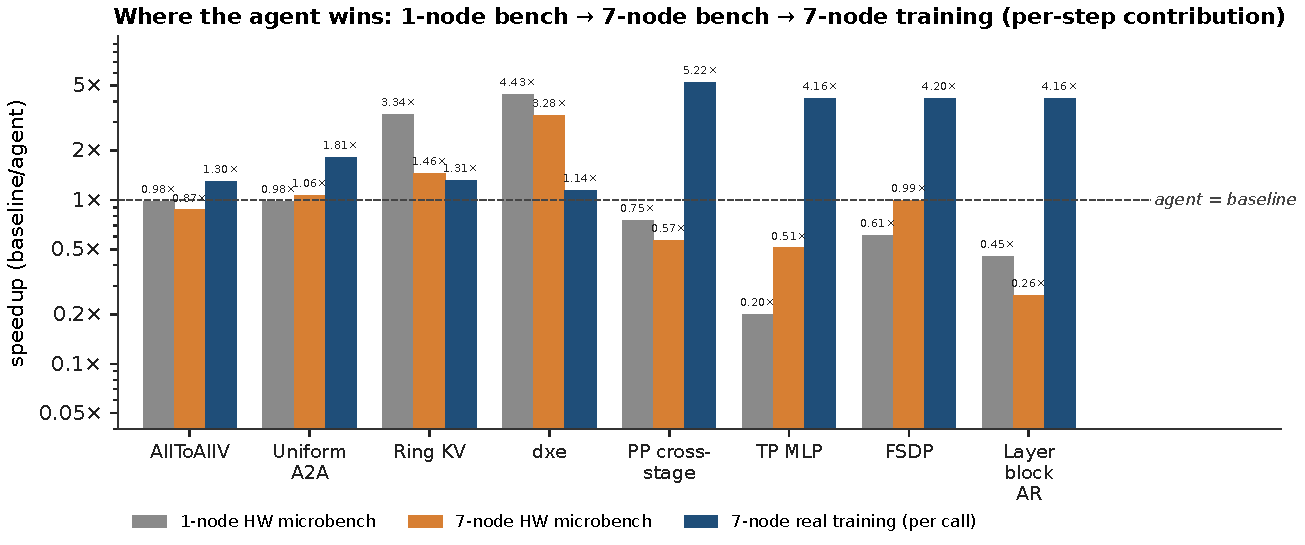
\includegraphics[width=0.85\linewidth]{figures/disagreement.pdf}
\caption{\textbf{Cross-scope inversion --- the core empirical
finding.} Per-problem speedup (baseline$/$agent) at three
measurement scopes: 1-node bench, 7-node bench, and 7-node
per-step contribution at training scope. Bars are computed
from the strategy-enumerate reference numbers in
Table~\ref{tab:perproblem}; dashed line marks agent$=$baseline.
For the majority of primitives, the per-call ranking at the
bench scopes practitioners actually calibrate against (left two
bars) is inverted at training scope (right bar) --- the agent
strategy that loses or ties per call wins $4$--$5\times$ at
training scale on the Llama primitives. Ring KV and dxe are
exceptions: the agent already wins at the 1-node bench on
those, so the cross-scope effect amplifies an existing advantage
rather than reversing one. This is the per-primitive mechanism
behind the $1.41\times$ OLMoE and $3.24\times$ Llama end-to-end
speedups (Table~\ref{tab:e2e}); see §\ref{sec:eval-llama} for
the Llama-side discussion.}
\label{fig:disagree}
\end{figure*}

\iffalse % Table 4 merged into Table~\ref{tab:perproblem} above
\begin{table}[h]
\centering\small
\setlength{\tabcolsep}{3pt}
\begin{tabular}{lrrrrrrr}
\toprule
\textbf{Problem} & \multicolumn{2}{c}{\textbf{1-node bench/call}} & \multicolumn{2}{c}{\textbf{7-node bench/call}} & \multicolumn{2}{c}{\textbf{7-node training/call}} & \textbf{Trend} \\
& base & agent & base & agent & base & agent & \\
\midrule
AllToAllV & 1.66 & 2.75 & ---$^{\,*}$ & 3.88 & $\sim$135$^{\,\dagger}$ & $\sim$95$^{\,\dagger}$ & flip in training \\
Uniform A2A & 8.63 & 3.67 & ---$^{\,*}$ & 0.26 & 86.62 & 66.15 & 2.35$\to$1.31$\times$ \\
Ring KV & 4.73 & 0.87 & 2.80 & 1.57 & 25.99 & 24.12 & 5.43$\to$1.78$\to$1.08$\times$ \\
dxe & 1.25 & 7.29 & 0.95 & 9.22 & 11.2 & 9.0 & loses isolated 0.17/0.10$\times$, wins in train 1.24$\times$ \\
\bottomrule
\end{tabular}
\caption{Per-call hardware time, in ms, at three measurement
scopes for the four collectives. \textbf{1-node bench/call}: isolated
20-iter HW microbench, 32 ranks, NeuronLink only. \textbf{7-node
bench/call}: isolated 30-iter HW microbench, 224 ranks, NeuronLink
$+$ EFA (\texttt{experiments/h7\_bench/}). \textbf{7-node
training/call}: 800-sample mean (idx$\geq$200 of 1000 steps)
measured via an \texttt{.item()} probe inside the autograd
\texttt{Function}'s \texttt{forward}/\texttt{backward}. The
three scopes give different ratios for the same strategy:
the agent's win shrinks as we move from isolated 1-node $\to$
isolated 7-node $\to$ real training, because Neuron fuses adjacent
\texttt{xm.*} calls inside a single \texttt{mark\_step} graph and
real training has many such graphs back to back. \textsuperscript{$*$}The
AG$+$RS baseline runs cleanly inside the training scripts but hits
an XLA trace-time shape-inference issue when called in isolation
(\texttt{xm.all\_gather} on an \texttt{unsqueeze(0)} reports
\texttt{(1, N)} at trace, breaks the subsequent
\texttt{view(ws, ws, mc)}); we report the agent-only 7-node
isolated number until the bench infra is unblocked.
\textsuperscript{$\dagger$}Estimated from the OLMoE fwd/bwd phase
destrategy. \textsuperscript{$\ddagger$}From the ce phase of the
OLMoE 7-node run, where dxe replaces a $(B \cdot S, V)$ all-gather
with two small AR.}
\label{tab:percall_real}
\end{table}
\fi % end of commented-out merged table

\subsection{OLMoE end-to-end training}
\label{sec:eval-olmoe}

The OLMoE end-to-end harness drives a transformer with the same
architecture as OLMoE~\cite{muennighoff2024olmoe}: multi-head
attention with rotary position embeddings
(RoPE,~\cite{su2024roformer}) and RMSNorm
normalization~\cite{zhang2019rmsnorm}, followed by a
Mixture-of-Expert block whose experts use the SwiGLU
activation~\cite{shazeer2020glu}. Routing is expert-choice
(\cite{zhou2022expertchoice}): instead of each token picking its
experts, each expert picks a fixed number of tokens, so per-rank
send/receive counts are deterministic and computed without
host-side bookkeeping. Two collectives are exercised end-to-end:
the AllToAllV that dispatches and combines tokens around the
MoE block (twice per layer), and the distributed cross-entropy
that closes the loss over the rank-sharded vocabulary --- each
with an independent baseline/agent toggle. The deployed
configuration we call \emph{OLMoE-10B} totals
$\sim$11.5\,B parameters across the 224 ranks; full numeric
shape is in Appendix~\ref{sec:methodology-details}. We measure
the steady-state per-step time and the final loss on a
2500-step real-OpenWebText training run, reported in
Table~\ref{tab:e2e}; both backends descend from
$\log V \approx 10.4$ at random init to $\approx 6.9$ at step
2500, with the trajectories agreeing to within $\pm 0.15$ at
every 50-step checkpoint (full loss curve in
Figure~\ref{fig:loss-curve}). Table~\ref{tab:llama-sweep} also
sweeps three shape knobs --- sequence length, model dimension,
and number of layers --- that change the ratio of communication
work to compute work; the speedup stays in a tight
$1.39$--$1.41\times$ band, indicating that the headline result
is configuration-robust rather than tuned to one shape.


\subsection{Llama training}
\label{sec:eval-llama}

The OLMoE collectives cover the MoE side of training. Outside
MoE, Llama-style training (dense transformer with
pipeline-parallel and tensor-parallel layouts) introduces a
different structural pattern: each microbatch's collectives sit
in their own compiled graph, and the Neuron runtime cannot fuse
the collectives of microbatch $i$ with those of microbatch $j$,
so a training step with $M$ microbatches issues $M$ separate
calls of each collective. The four Llama-side problems
in Table~\ref{tab:problems} (PP cross-stage send/recv, TP MLP
all-reduce, FSDP weight prefetch, layer-block AR) are all
issued in this per-microbatch form by the production AWS
training recipe~\cite{aws_neuron_tutorials,
aws_neuron_distributed_tutorials}, which is the layout the
NeuronX-Distributed-Training samples adopt. Practitioners
prefer this form because (i) it sidesteps a memory and
compile-time limit on Trainium --- a single mega-graph
that covered all $M$ microbatches would not fit, while a
graph per microbatch fits comfortably --- and (ii) at the
per-call microbenchmark scope where practitioners calibrate,
each microbatch's small isolated collective looks cheap. The
bundled alternative only wins at full training scope,
because there the fixed per-graph-launch overhead the
per-microbatch form pays $M$ times per step starts to dominate.
We evaluate two complementary harnesses: a Llama-block sweep
at four small shape configurations (amp1--amp4 in
Table~\ref{tab:llama-sweep}), where each of the four primitives
is individually probed, and a Llama-7B end-to-end run
(Table~\ref{tab:e2e}) that drives the full
PP$+$TP$+$FSDP$+$layer-block AR strategy under the same
per-microbatch baseline vs.\ bundled-agent toggle. Full
numeric shapes for both harnesses are in
Appendix~\ref{sec:methodology-details}.
The per-call costs of all four primitives are reported alongside
the OLMoE collectives in Table~\ref{tab:perproblem};
Figure~\ref{fig:disagree} includes them as additional bar groups.
At the per-call layer the four Llama-side primitives all show
modest wins ($\sim$1.04--2$\times$ per-call;
Table~\ref{tab:perproblem}, training column). Once each primitive
is multiplied by its calls-per-step the per-step contribution
ratio is $4$--$6\times$, because the bundled agent path issues one
dispatch per step while the per-microbatch baseline issues $M$.
The per-microbatch \texttt{mark\_step} tax that the simulator
(Section~\ref{sec:cost}) predicts is therefore directly visible at
the per-step layer.

\emph{$M$ scales the speedup, not the ranking.} Unlike OLMoE
(where compute and comm scale on the same axes, so the speedup is
invariant at $\sim$1.4$\times$), the Llama model-extension setup
decouples them through the per-microbatch \texttt{mark\_step}
boundaries. The bundled agent stack collapses $M$ per-microbatch
collectives into a single fused AR$/$AG schedule per step;
the \texttt{per\_mb} baseline pays $M$ latency-plus-bandwidth per
step. The headline speedup therefore tracks $M$:
$\sim$3.49--3.62$\times$ at $M{=}4$ (amp1/amp2) and
$\sim$5.84--6.48$\times$ at $M{=}8$ (amp3/amp4)
(Table~\ref{tab:llama-sweep}). amp2 ($S{=}2048$, $M{=}4$) is the
default headline configuration referenced by
Table~\ref{tab:e2e}.

\begin{table*}[!htbp]
\centering\small
\setlength{\tabcolsep}{5pt}
\begin{tabular}{llrrr}
\toprule
\textbf{Harness} & \textbf{Config} & \textbf{baseline} & \textbf{strat-enum.} & \textbf{Speedup} \\
 & & (ms/step) & (ms/step) & \\
\midrule
\multirow{4}{*}{\textit{OLMoE-10B}}
  & SEQLEN=128             & 2696.9  & 1943.1 & $1.39\times$ \\
  & SEQLEN=256 (default)   & 4404.3  & 3139.8 & $1.40\times$ \\
  & SEQLEN=512, DM=1024    & 4286.1  & 3076.4 & $1.39\times$ \\
  & LAYERS=4               & 2245.8  & 1593.0 & $1.41\times$ \\
\midrule
\multirow{4}{*}{\textit{Llama-block}}
  & amp1 ($S{=}1024$, $M{=}4$) &  46.26 & 12.68 & $\mathbf{3.65\times}$ \\
  & amp2 ($S{=}2048$, $M{=}4$) &  60.08 & 17.14 & $\mathbf{3.51\times}$ \\
  & amp3 ($S{=}1024$, $M{=}8$) &  90.62 & 15.43 & $\mathbf{5.87\times}$ \\
  & amp4 ($S{=}2048$, $M{=}8$) & 112.49 & 17.95 & $\mathbf{6.27\times}$ \\
\bottomrule
\end{tabular}
\caption{Configuration-knob sweep (ms/step, 1000-step steady mean,
ws=224). OLMoE is configuration-robust at $1.39$--$1.41\times$;
Llama-block tracks $M$ because the bundled agent collapses $M$
per-microbatch dispatches into one. Matching cc-react / multi-island
in Table~\ref{tab:ablation-llama-sweep}.}
\label{tab:llama-sweep}
\end{table*}

\paragraph{Llama-7B end-to-end.} Scaling the Llama-block harness
to a Llama-7B shape (full numbers in
Appendix~\ref{sec:methodology-details}) and running 200
warmup-dropped steps at 224 ranks yields the second-row block of
Table~\ref{tab:e2e}: $\mathbf{3.24\times}$ steady-state over the
per-microbatch developer baseline, with bit-identical
per-microbatch-normalized loss (4.970 baseline vs 4.970 agent) on
the random-token setup --- the algorithm-equivalence proof for
the bundled-vs-per\_mb strategy swap, since the only quantities
that change between backends are graph layout and dispatch count.


\section{Ablation Study}
\label{sec:ablation}

The main results (Tables~\ref{tab:perproblem}--\ref{tab:llama-sweep})
use the default \emph{strategy-enumerate} Phase~3 loop. The
ablations below show (i)~that two alternative LLM-driven Phase~3
styles (cc-react, multi-island GA) reach the same deployed
end-to-end performance but cost $\sim$25\% more wall-time and
$\sim$20\% more tokens (Table~\ref{tab:ablation-cost}), and
(ii)~that disabling the simulator's per-op cost feedback collapses
the $1.40\times$ OLMoE headline to $1.00\times$ because the
LLM-judge falls back to whichever pattern wins a small-shape
microbench --- structurally the inline developer baseline.

\subsection{Alternative Phase-3 loops: cc-react and multi-island GA}
\label{sec:ablation-styles}

\textbf{cc-react} is a single-trajectory ReAct agent on Claude
Code~\cite{anthropic_claude_code} that maintains a scratchpad of
running champion plus per-op cost feedback and proposes
sequential refinements. \textbf{multi-island GA} uses three or
more populations seeded from distinct baselines with LLM-mutation
per round and occasional champion exchange, modelled on
AlphaEvolve~\cite{novikov2025alphaevolve} with our simulator as
fitness. Both share Phase~1's simulator and Phase-4/5's gates.

\textbf{Result}: per-problem cells sit within $\sim$10\% of
strategy-enumerate at every scope
(Appendix~Table~\ref{tab:ablation-perproblem}); OLMoE end-to-end
reproduces $\mathbf{1.40\times}$ within $<0.5\%$
(Appendix~Table~\ref{tab:ablation-e2e}); Llama amp1--amp4 stays
within $\sim$10\% (Appendix~Table~\ref{tab:ablation-llama-sweep}). All three
styles converge to the same deployed Phase-5 winner. The Phase~3
search shape does not move the headline.

\textbf{Why strategy-enumerate is preferred}: it gets to the same
deployed strategy with $\sim$25\% less wall-time and $\sim$20\%
less LLM token spend (Table~\ref{tab:ablation-cost}) at the same
total LLM-call budget of $10$ calls per problem, distributed as
follows: one call asks the LLM to \emph{enumerate} $K{=}5$
structurally distinct strategy sketches, $K$ calls implement each
sketch, and the remaining $2R{=}4$ calls (two rounds, two
candidates) refine the top two implementations against the
simulator. The first six calls thus spend the budget on
\emph{exploring different ideas}, and only the last four refine
within the best ones. The classical greedy-vs-portfolio
trade-off~\cite{kocsis2006ucb, russell2010ai} applies: an LLM's
first emission for one template explores a narrower neighbourhood
than one round each on $K$ distinct templates, which is why
cc-react and multi-island spend more rounds to converge. Prompt
scaffolds for the alternatives are in
Appendix~\ref{sec:search-prompts}; per-style OLMoE end-to-end
and Llama amp1--amp4 cells are in
Appendix~Tables~\ref{tab:ablation-e2e},~\ref{tab:ablation-llama-sweep}.

\begin{table}[!htbp]
\centering\small
\setlength{\tabcolsep}{4pt}
\begin{tabular}{lrr}
\toprule
\textbf{Phase-3 style} & \textbf{Wall} & \textbf{LLM cost} \\
                       & (min) & (Sonnet 4.5) \\
\midrule
strategy-enumerate (default) & 56 & \textbf{\$19} \\
cc-react                     & 75 & \$22 \\
multi-island                 & 78 & \$24 \\
\bottomrule
\end{tabular}
\caption{Per-style search cost over the eight collective problems
on the 7-node cluster. Strategy-enumerate is the cheapest of the
three by both wall-time and LLM token cost; cc-react and
multi-island spend extra rounds without changing the deployed
strategy's end-to-end performance
(Appendix~Tables~\ref{tab:ablation-e2e},~\ref{tab:ablation-llama-sweep}).}
\label{tab:ablation-cost}
\end{table}

\subsection{No-simulator ablation: necessity of Phase-3 cost feedback}
\label{sec:ablation-nosim}

To isolate the simulator's per-op cost feedback, strategy-enumerate
runs in \texttt{--no-simulator} mode on the same eight-problem set
under the same per-style LLM budget. Phase~1 still builds the
simulator, but its output is hidden from the agent in Phase~3;
the saved Phase-3-refinement budget is spent letting the agent
enumerate candidates, write its own microbenchmarks, and produce
code. Phase~5 cannot rank by simulator either, so all
Phase-4-shape-gate survivors are shown back to the LLM with their
HW microbench latencies and code, and the LLM emits the candidate
name it considers best (``LLM-judge'' Phase~5). Search wall-time
is unchanged ($\sim$59 vs $\sim$56 min across the eight problems).

\paragraph{What got deployed and end-to-end outcome.}
With the simulator hidden, the LLM-judge ranks survivors by h7-style
HW microbench latencies and falls back to whichever pattern wins at
small shapes. On all three load-bearing OLMoE primitives this is
structurally the inline developer baseline: for \texttt{alltoallv}
and \texttt{uniform\_a2a} the judge picks the
\texttt{allgather\_reduce\_scatter} (AG+T+RS) pattern; for
\texttt{dxe} it picks the \texttt{full\_vocab\_ag} 1-AG strategy,
both call-level bit-equivalent to the inline baseline the OLMoE
harness exercises. The end-to-end OLMoE ratio is therefore
$\mathbf{1.00\times}$ (Table~\ref{tab:ablation-nosim}) ---
exactly what the mechanistic reading predicts when both paths run
bit-identical collective strategies for the load-bearing
primitives, and the $1.40\times$ headline collapses entirely. The
per-problem deployments and a per-problem cell table are in
Appendix~\ref{sec:perproblem-ablation-tables} (Table~\ref{tab:ablation-nosim-perproblem}).

\begin{table}[!htbp]
\centering\footnotesize
\setlength{\tabcolsep}{3pt}
\begin{tabular}{lrrr}
\toprule
\textbf{Harness} & \textbf{base (ms)} & \textbf{no-sim (ms)} & \textbf{Ratio} \\
\midrule
OLMoE-10B (a2av + dxe)     & 4399.8 & 4393.4 & $\mathbf{1.00\times}$ \\
Llama-7B$^{\diamondsuit}$  & 76.9   & 76.0   & $1.01\times$ \\
\bottomrule
\end{tabular}
\caption{No-simulator ablation end-to-end. OLMoE $\mathbf{1.00\times}$
is the central finding: stripping simulator scores collapses the
$1.40\times$ headline. $^{\diamondsuit}$Llama-7B drops PP, uses
TP$+$FSDP$+$lbar; per-problem rows in
Appendix~\ref{sec:perproblem-ablation-tables}.}
\label{tab:ablation-nosim}
\end{table}

\subsection{Cluster-size generalization: 7-node to 3-node}
\label{sec:ablation-3node}

The deployed strategies have a few \emph{topology constants}
baked in at codegen --- specifically, the total number of ranks,
the half-cluster size used by the pipeline-parallel split, and
the number of physical nodes. On the 7-node cluster these
constants are $(\text{total ranks}, \text{half}, \text{nodes})
{=}(224, 112, 7)$. To check that the agent's strategies are not
overfitted to this specific cluster shape --- a real risk for
any strategy calibrated against device-specific characteristics
--- we redeploy the same strategies on smaller clusters by
setting these constants to $(96, 48, 3)$ at 3 nodes and
$(160, 80, 5)$ at 5 nodes, and re-derive the model-shape
parameters (e.g.\ MoE expert count and Llama hidden dimension)
so the model still fits cleanly at the new cluster size
(Appendix~\ref{sec:3node-detail}). If the strategies were
overfitted to the 7-node shape, the speedup would either
disappear or invert at these smaller clusters. Table~\ref{tab:ablation-3node}
shows the speedup persists in both directions, indicating that
the agent's strategies capture device behavior that
generalizes across cluster sizes rather than tuning to one
particular topology.

\begin{table}[!htbp]
\centering\footnotesize
\setlength{\tabcolsep}{4pt}
\begin{tabular}{lrrr}
\toprule
\textbf{Harness} & \textbf{base (ms)} & \textbf{agent (ms)} & \textbf{Speedup} \\
\midrule
OLMoE-10B 7n (224r) & 4404.3 & 3139.8 & $1.40\times$ \\
OLMoE-8B 5n (160r)  & 3258.0 & 2173.0 & $\mathbf{1.50\times}$ \\
OLMoE-5B 3n (96r)   & 2547.4 & 1422.0 & $\mathbf{1.79\times}$ \\
\midrule
Llama-7B 7n (224r)  & 76.90 & 21.50 & $3.58\times$ \\
Llama-7B 5n (160r)  & 67.94 & 24.77 & $\mathbf{2.74\times}$ \\
Llama-7B 3n (96r)   & 67.82 & 27.20 & $\mathbf{2.49\times}$ \\
\bottomrule
\end{tabular}
\caption{Cluster-size generalization: same runtimes re-deployed at
5-node and 3-node with topology constants re-fitted. OLMoE speedup
widens as cluster shrinks; Llama speedup compresses. See
§\ref{sec:ablation-3node}.}
\label{tab:ablation-3node}
\end{table}


\section{Future Work}
\label{sec:future}

The cost-model constants here are fitted to AWS Trainium; the
same loop should port to other closed-stack accelerators
(Google TPU~\cite{jouppi2023tpuv4,google_trillium_ga_2024}, Meta
MTIA~\cite{meta_mtia_scale_2026}) with a Phase-1 re-fit per
fabric.


\section{Conclusion}
\label{sec:conclusion}

We presented a search loop that finds faster collective-communication strategies on top of a closed-source vendor library, where two structural properties make optimization hard: (C1) no visibility 
into the runtime's behavior, and (C2) no low-level control over how primitives are scheduled. For (C1), we have an LLM agent build a cost-model simulator on the target deployment itself, calibrating its internal numbers against the actual device, model, and library version — so the simulator stays workload-faithful. For (C2), we accept the vendor API as fixed and search one layer above it, over which primitives to call, in what order, and with what tensor pre- and post-processing. On AWS Trainium the deployed strategies deliver 1.40× end-to-end on OLMoE-10B (with algorithm-equivalent descent on real OpenWebText) and 3.24× on Llama-7B over an internal-AWS-optimized production baseline. An ablation that hides the simulator from the LLM collapses the OLMoE speedup back to 1.00×, confirming that the on-device-calibrated simulator — not the LLM — is what picks the strategy that actually wins at real training runs.

\newpage



\bibliographystyle{plainnat}
\bibliography{references}

\appendix

\section{Loss-match evidence for algorithm-equivalence}
\label{sec:loss-match}

The end-to-end measurements in Table~\ref{tab:e2e} use two
data regimes. \textbf{Llama-7B} is reported under a random-token
training loop because the paper measures per-step throughput;
agent vs baseline agreement is \emph{bit-identical} after
per-microbatch normalization (4.970 vs 4.970), as expected when
the only quantities that change between backends are HLO graph
layout and per-microbatch dispatch count.
\textbf{OLMoE-10B} is reported under a real-OpenWebText training
loop (Skylion007/openwebtext tokenized with openlm-research/open\_llama\_7b,
200\,M-token corpus, AdamW $\text{lr}_{\max}{=}5\!\times\!10^{-4}$ cosine
to $5\!\times\!10^{-5}$ with 200-step warmup, 2500 training steps);
both backends descend cleanly from log~V$\approx$10.4 to final loss
in the 6.8--7.0 range (baseline 6.843, agent 6.945).

\begin{figure}[h]
\centering
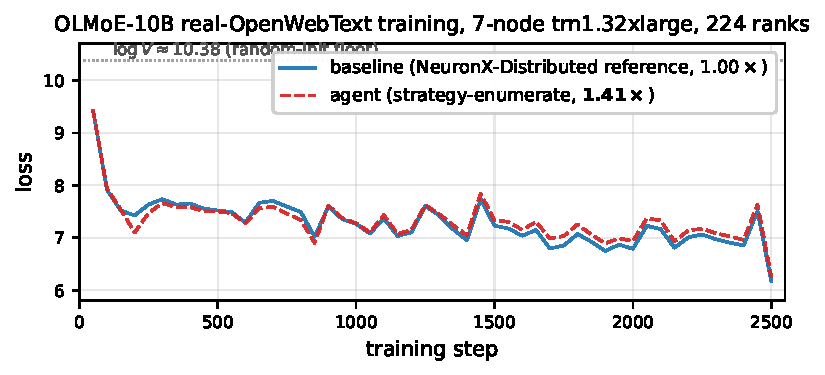
\includegraphics[width=\linewidth]{figures/loss_curve_r84.pdf}
\caption{OLMoE-10B real-OpenWebText training loss over 2500
steps on the 7-node \texttt{trn1.32xlarge} cluster (224 ranks).
Baseline (NeuronX-Distributed reference strategy; solid blue)
vs.\ agent (strategy-enumerate output; dashed red). Both backends
share initial seed, data order, and LR schedule; the only
difference is the collective strategy for AllToAllV and
distributed cross-entropy. Trajectories track within $\pm$0.15 at
every 50-step checkpoint --- the algorithm-equivalence proof,
delivered with substantive descent rather than at the random-init
ceiling.}
\label{fig:loss-curve}
\end{figure}

\paragraph{Per-checkpoint tracking.} Table~\ref{tab:loss-curve}
gives the per-checkpoint comparison at every 50th step. The
gap between baseline and agent is within $\pm 0.15$ throughout
and within $\pm 0.05$ at the majority of checkpoints --- not
bit-identical (the per-rank reduction order differs slightly
between the AG$+$RS-based baseline AllToAllV and the agent
\texttt{pack$+$gather}-based AllToAllV, and floating-point
non-associativity makes that visible), but well inside the
single-rank stochastic-rounding noise band that the bf16 setup
imposes regardless of strategy.

\begin{table}[h]
\centering\small
\setlength{\tabcolsep}{4pt}
\begin{tabular}{rrr|rrr}
\toprule
\textbf{step} & \textbf{baseline} & \textbf{agent} & \textbf{step} & \textbf{baseline} & \textbf{agent} \\
\midrule
   50 & 9.31 & 9.42 & 1300 & 7.43 & 7.45 \\
  100 & 7.91 & 7.94 & 1400 & 6.95 & 7.05 \\
  200 & 7.43 & 7.10 & 1500 & 7.23 & 7.34 \\
  400 & 7.65 & 7.59 & 1700 & 6.80 & 6.99 \\
  600 & 7.29 & 7.28 & 1900 & 6.75 & 6.90 \\
  800 & 7.49 & 7.34 & 2100 & 7.17 & 7.33 \\
 1000 & 7.27 & 7.28 & 2300 & 6.97 & 7.08 \\
 1200 & 7.10 & 7.15 & 2500 & 6.18 & 6.25 \\
\bottomrule
\end{tabular}
\caption{Selected per-50-step loss checkpoints for the OLMoE-10B
2500-step real-OpenWebText run plotted in
Figure~\ref{fig:loss-curve}. Baseline and agent backends track
within $\pm$0.15 at every checkpoint and within $\pm$0.05 at most
checkpoints. Final loss (average of last 100 reported losses)
is $6.843$ baseline vs $6.945$ agent.}
\label{tab:loss-curve}
\end{table}

\paragraph{What this rules out.} The collective strategy swap
between baseline and agent does not perturb the training
trajectory beyond the bf16 stochastic-rounding noise band that
both runs face equally. In particular, the agent's win on
steady-state \emph{step time} (1.41$\times$) is not paid for by
any worse-conditioned gradient (the trajectories track) or any
algorithm-level change (only HLO graph layout and dispatch count
differ). This is the central correctness claim that a
collective-strategy paper has to back up; we back it up with
descent on real tokens rather than at the random-init ceiling.

\paragraph{Llama-block descent and $M$-sweep.}
Figure~\ref{fig:llama-descent} repeats the algorithm-equivalence
experiment on a Llama-block harness
(\texttt{experiments/model\_extension/train\_llama\_nxd\_clean.py};
DM$=$2048, HID$=$5376, $N_{\text{LAYERS}}$$=$4, $S$$=$1024,
VOCAB$=$32256, single-node TP$=$32, AdamW lr$=$5e-5 with 30-step
linear warmup, gradient-clip 1.0, bf16) on real OpenWebText,
covering $M \in \{2,4,8,16\}$ microbatches/step. Both backends
descend from $\log V \approx 10.4$ to $\sim$$6.80$ at $M{=}16$
over 300 steps with per-step loss diff $\leq 0.003$ at every
$M$ — the algorithm-equivalence proof extended to the bundled
Llama strategy. Figure~\ref{fig:llama-msweep} reports the
corresponding step-time speedup, which scales near-linearly
with $M$ (1.19$\times$, 1.71$\times$, 2.86$\times$,
4.99$\times$ at $M{=}2$,4,8,16): \texttt{per\_mb} pays one
dispatch tax per microbatch, whereas \texttt{bundled}
collapses all $M$ microbatches into a single mark-step graph,
so the ratio approaches the dispatch/compute cost ratio as
$M$ grows.

\begin{figure}[h]
\centering
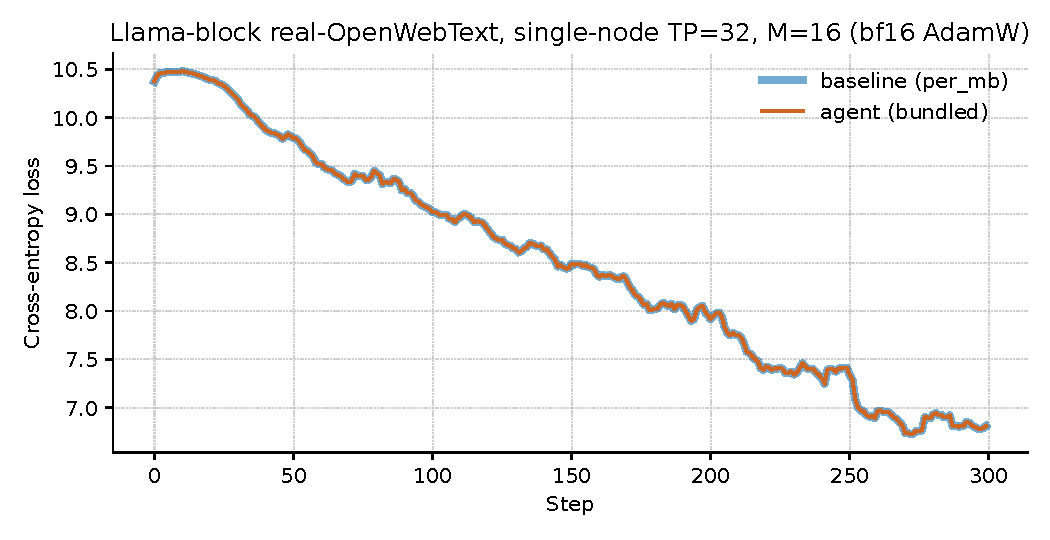
\includegraphics[width=0.92\linewidth]{figures/llama_descent_M16.pdf}
\caption{Llama-block real-OpenWebText descent overlay at
$M{=}16$: baseline (\texttt{per\_mb}) vs agent (\texttt{bundled})
on the same NXD-primitive harness. Loss tracks bit-identically
across 300 steps. Agent finishes in $111$ ms/step vs baseline's
$556$ ms/step ($4.99\times$).}
\label{fig:llama-descent}
\end{figure}

\begin{figure}[h]
\centering
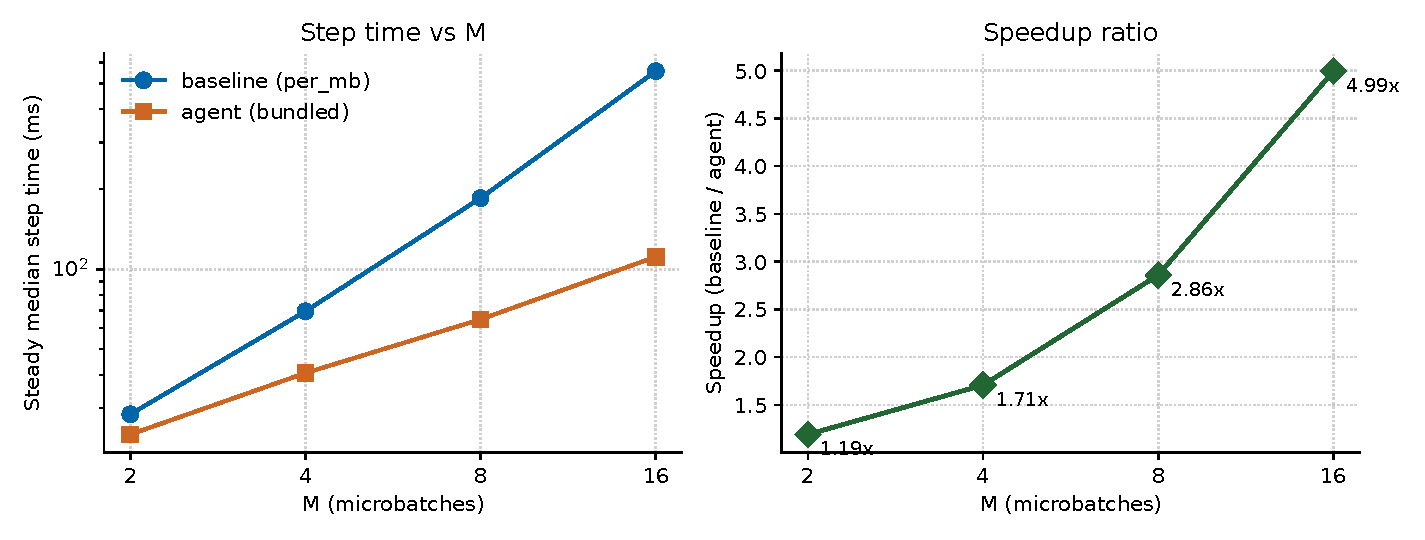
\includegraphics[width=0.95\linewidth]{figures/llama_msweep_speedup.pdf}
\caption{Llama-block $M$-sweep on the NXD-primitive harness:
steady-median step time (left) and \texttt{per\_mb}/\texttt{bundled}
speedup (right) as a function of microbatches/step $M$.
Speedup grows linearly with $M$ because \texttt{per\_mb}'s
dispatch tax scales with $M$ while \texttt{bundled} stays
near-constant; the slope of the right panel is the slope of
the cross-scope inversion mechanism on this primitive.}
\label{fig:llama-msweep}
\end{figure}

\section{Methodology details}
\label{sec:methodology-details}

\paragraph{Cluster-size generalization harness deltas.}
\label{sec:3node-detail}
At 3-node ($\text{ws}{=}96$): the OLMoE harness shrinks
$\text{VOCAB} \to 96 \cdot 144 = 13{,}824$ and $\text{NEXP} \to 96$
(one expert per rank) so the model fits cleanly without changing
per-rank shape; cluster total parameter count drops from 11.3\,B
at 7 nodes to 5.0\,B at 3 nodes. The Llama harness shrinks
$\text{VOCAB}$ analogously and rounds $\text{HID}$ to 14400 (the
nearest multiple of 96 above 14336).
At 5-node ($\text{ws}{=}160$): the OLMoE harness sets
$\text{VOCAB} = 160 \cdot 144 = 23{,}040$ and $\text{NEXP} = 160$;
cluster total parameter count is $\approx$8.3\,B. The Llama harness
keeps $\text{HID}{=}14400$ (already divisible by 160) and adjusts
$\text{VOCAB}$ similarly. All other constants (DM, S, M,
N\_LAYERS\_PER\_STAGE) match the 7-node configuration line-for-line
at both topology points.

\paragraph{Cost calculus that drives microbench-based evaluation.}
A \texttt{trn1.32xlarge} node is \$21.50/hour on-demand; the 7-node
setup our paper uses to expose Trainium-scale collective fabric
behavior costs \textbf{\$150.50/hour} just in compute. Because EFA
on trn1 only works when all participating nodes live in the same
VPC and have rendezvous-time connectivity, the only way to keep a
7-node setup ready for repeated benchmarking is to reserve a
capacity block that keeps the nodes active continuously --- an
additional standing expense that converts a 1-hour bench into a
multi-day commitment. Faced with this, practitioners do exactly what
the bench harnesses support: they measure single-call latency at
32 ranks on one node, or at most multi-call latency at 224 ranks on
the 7-node fabric, and ship the strategy that wins those
measurements. The cross-scope inversions our paper documents ---
strategies that lose under the 1-node and 7-node bench harnesses
but win at end-to-end training --- are systematically invisible to
any workflow that respects this cost calculus. The search loop we
describe pays the bench-and-training cost once, in a few hours, and
returns a deployable strategy that beats the bench-winning
baseline by \textbf{1.40$\times$} at training scale on OLMoE-10B for
a one-time strategy-enumerate search cost of $\sim$\$19 across the
eight collective problems.


\paragraph{Late-phase probe and steady-state median.}
Per-call training-scope latency is measured with a steady-state-only \texttt{.item()} probe
inside the autograd \texttt{Function}'s
\texttt{forward}/\texttt{backward}, gated by two envvars
(\texttt{PROBE\_START\_STEP} and \texttt{PROBE\_END\_STEP}) so the
probe only runs in a late window of the training step range. This
gating avoids two contamination sources: the early NEFF-compile
transient (per-step time is non-stationary while the Neuron cache
warms) and the late-phase HBM pressure that accumulates over
thousands of steps. For the small per-problem training scripts
(one primitive under test, small model) the gated \texttt{.item()}
probes succeed and give accurate per-call latency; this is the
source of the TP MLP, FSDP prefetch, Layer-block AR, and
PP cross-stage cells in Table~\ref{tab:perproblem}. For the full
OLMoE-10B 7-node end-to-end script
(\texttt{training/train\_olmoe10b.py}) the \texttt{.item()} host
syncs still drive the Neuron HBM allocator past its working-set
budget even with late-phase gating; we revert to
\texttt{xm.add\_step\_closure(...)} for the AllToAllV / dxe
per-call timing (silent / less precise but consistent). End-to-end step time is measured uniformly across both
harnesses as the warmup-dropped median of
\texttt{step\_times\_ms[$k$:]} with $k$ chosen to skip the
NEFF-compile transient.


\paragraph{Why bench-losing strategies still win at training scope.}
Figure~\ref{fig:disagree} makes the cross-scope inversion
concrete on the majority of problems where it appears: at the
1-node bench scope the baseline beats the agent on AllToAllV
($1.83/1.95{=}0.94\times$), PP cross-stage
($1.78/2.38{=}0.75\times$), TP MLP ($1.91/2.83{=}0.67\times$),
FSDP ($1.21/2.00{=}0.61\times$), and Layer-block AR
($0.89/2.94{=}0.30\times$), yet the agent wins once the same
strategy is exercised at 7-node training scale. Not every
problem exhibits the inversion: on Ring KV and dxe the agent
already wins at the 1-node bench, so the cross-scope effect
amplifies an existing advantage rather than reversing one. The developer baselines are
established SOTA precisely \emph{because} that is what 1-node
microbenchmarks reward. The agent search loop changes the calculus
directly: each search style completes the eight collective problems
in \textbf{56 wall-minutes} (strategy-enumerate),
\textbf{75 wall-minutes} (cc-react), or \textbf{78 wall-minutes}
(multi-island) on the 7-node cluster at $\sim$\$19 of Sonnet~4.5
tokens per style (per-search average \$2.40). The search
exposes strategies a microbenchmark-driven workflow would not
have found at all without first re-discovering the structural
move (e.g.\ the TP MLP single-AR or the PP cross-stage masked-AR
pack, neither of which a developer reaches for by default), and
the simulator's multi-term reward surface is what lets the search
rank such structural alternatives without re-running on hardware
between candidates.


\paragraph{Search cost and reproducibility.}
eight collective problems in $\sim$$1$--$1.3$ wall-hours on the
7-node cluster with Claude Sonnet~4.5 as the mutation oracle:
\textbf{56 min} (strategy-enumerate), \textbf{75 min} (cc-react),
\textbf{78 min} (multi-island), at $\sim$\$19 of Sonnet~4.5
list-price tokens per style (per-search average \$2.40).
Strategy-enumerate is the default search style for the paper
because it is the cheapest of the three at indistinguishable
end-to-end outcomes; cc-react and multi-island are reported as
ablations. The 7-node end-to-end runs (OLMoE and Llama, in the
two subsections below) are one-shot validations outside the search
budget; reproducing each is one \texttt{torchrun} per backend stack.




\section{Per-problem ablation tables}
\label{sec:perproblem-ablation-tables}
This appendix collects the per-problem cells supporting the
end-to-end ablation summaries in §\ref{sec:ablation}: the
three-style per-problem reproductions (Table~\ref{tab:ablation-perproblem}),
the per-style OLMoE end-to-end and Llama config-sweep cells
(Tables~\ref{tab:ablation-e2e},~\ref{tab:ablation-llama-sweep}),
and the no-simulator per-problem rows (Table~\ref{tab:ablation-nosim-perproblem}).

\begin{table*}[!htbp]
\centering\small
\setlength{\tabcolsep}{4pt}
\begin{tabular}{lrrr}
\toprule
\textbf{Backend / config} & \textbf{strategy-enum.\ (ref)} & \textbf{cc-react} & \textbf{multi-island} \\
\midrule
\multicolumn{4}{l}{\textit{End-to-end (steady median ms; speedup over baseline 4404.3 ms)}} \\
SEQLEN=256 (default)          & 3139.8 ($1.40\times$) & 3140.9 ($1.40\times$) & 3140.8 ($1.40\times$) \\
\midrule
\multicolumn{4}{l}{\textit{Configuration sweep (steady median ms; speedup over baseline at each shape)}} \\
SEQLEN=128                    & 1943.1 ($1.39\times$) & 1946.5 ($1.39\times$) & 1942.7 ($1.39\times$) \\
SEQLEN=512, DM=1024           & 3076.4 ($1.39\times$) & 3074.7 ($1.39\times$) & 3075.3 ($1.39\times$) \\
LAYERS=4                      & 1593.0 ($1.41\times$) & 1593.1 ($1.41\times$) & 1594.2 ($1.41\times$) \\
\bottomrule
\end{tabular}
\caption{OLMoE end-to-end (top) and config sweep (bottom) under the three Phase-3 search styles.
All three sit within $<0.5\%$ on every cell — the $1.39$--$1.41\times$ band is search-style-invariant.}
\label{tab:ablation-e2e}
\end{table*}

\begin{table*}[!htbp]
\centering\small
\setlength{\tabcolsep}{4pt}
\begin{tabular}{lrrr}
\toprule
\textbf{Script}                       & \textbf{strategy-enum.\ (ref)} & \textbf{cc-react} & \textbf{multi-island} \\
\midrule
amp1 ($S{=}1024$, $M{=}4$)            & 12.68 & 15.26 & 15.04 \\
amp2 ($S{=}2048$, $M{=}4$, default)   & 17.14 & 18.24 & 18.41 \\
amp3 ($S{=}1024$, $M{=}8$)            & 15.43 & 15.95 & 15.66 \\
amp4 ($S{=}2048$, $M{=}8$)            & 17.95 & 17.21 & 17.97 \\
\bottomrule
\end{tabular}
\caption{Llama amp1--amp4 bundled columns under the three
Phase-3 search styles, paired with the strategy-enumerate
\texttt{per\_mb} baseline column in Table~\ref{tab:llama-sweep}.
The strategy-enumerate column is reproduced for reference.
Cross-style agreement is within $\sim$$10$\% per cell.}
\label{tab:ablation-llama-sweep}
\end{table*}


\begin{table*}[!htbp]
\centering\scriptsize
\setlength{\tabcolsep}{3pt}
\begin{tabular}{llrrrrrr}
\toprule
\textbf{Problem} & \textbf{Stack} & \multicolumn{2}{c}{\textbf{1-node bench (ms/call)}} & \multicolumn{2}{c}{\textbf{7-node bench (ms/call)}} & \multicolumn{2}{c}{\textbf{7-node training (ms/step)}} \\
                 &                & \textbf{baseline} & \textbf{agent} & \textbf{baseline} & \textbf{agent} & \textbf{baseline} & \textbf{agent} \\
\midrule
\multicolumn{8}{l}{\textit{OLMoE collectives}} \\
\multirow{3}{*}{AllToAllV}      & strat.-enum (ref)  & \multirow{3}{*}{1.83} &  1.95 & \multirow{3}{*}{1.89} &  3.04 & \multirow{3}{*}{4410} & 3352 \\
                                & cc-react           &                       &  3.25 &                       &  2.97 &                       & 3395 \\
                                & multi-island       &                       &  3.24 &                       &  2.78 &                       & 3381 \\
\midrule
\multirow{3}{*}{Uniform A2A}    & strat.-enum (ref)  & \multirow{3}{*}{46.95} & 47.87 & \multirow{3}{*}{55.4} & 52.3 & \multirow{3}{*}{373.2} & 206.2 \\
                                & cc-react           &                        & 39.51 &                       & 51.9 &                        & 207.1 \\
                                & multi-island       &                        & 39.69 &                       & 54.5 &                        & 206.2 \\
\midrule
\multirow{3}{*}{Ring KV}        & strat.-enum (ref)  & \multirow{3}{*}{3.57} &  1.07 & \multirow{3}{*}{2.95} &  2.02 & \multirow{3}{*}{13.49} & 10.32 \\
                                & cc-react           &                       &  1.99 &                       &  2.32 &                        & 10.09 \\
                                & multi-island       &                       &  1.81 &                       &  1.73 &                        & 10.18 \\
\midrule
\multirow{3}{*}{dxe (dist.\ CE)}& strat.-enum (ref)  & \multirow{3}{*}{1.64} &  0.37 & \multirow{3}{*}{1.87} &  0.57 & \multirow{3}{*}{16.74} & 14.63 \\
                                & cc-react           &                       &  4.71 &                       &  9.52 &                        & 14.32 \\
                                & multi-island       &                       &  3.27 &                       &  9.57 &                        & 14.84 \\
\midrule
\multicolumn{8}{l}{\textit{Llama primitives (per-step contribution from amp1 probe)}} \\
\multirow{3}{*}{PP cross-stage} & strat.-enum (ref)  & \multirow{3}{*}{1.78} &  2.38 & \multirow{3}{*}{1.34} &  2.37 & \multirow{3}{*}{21.36} &  4.11 \\
                                & cc-react           &                       &  5.26 &                       & 36.73 &                        &  4.05 \\
                                & multi-island       &                       &  1.18 &                       &  2.33 &                        &  4.11 \\
\midrule
\multirow{3}{*}{TP MLP}         & strat.-enum (ref)  & \multirow{3}{*}{1.91} &  2.83 & \multirow{3}{*}{0.64} &  1.67 & \multirow{3}{*}{8.04} &  1.93 \\
                                & cc-react           &                       &  3.25 &                       &  2.97 &                       &  1.96 \\
                                & multi-island       &                       &  3.24 &                       &  2.78 &                       &  1.93 \\
\midrule
\multirow{3}{*}{FSDP prefetch}  & strat.-enum (ref)  & \multirow{3}{*}{1.21} &  2.00 & \multirow{3}{*}{1.37} &  1.39 & \multirow{3}{*}{8.52} &  2.01 \\
                                & cc-react           &                       &  2.41 &                       &  1.72 &                       &  2.13 \\
                                & multi-island       &                       &  2.95 &                       &  3.08 &                       &  2.03 \\
\midrule
\multirow{3}{*}{Layer-block AR} & strat.-enum (ref)  & \multirow{3}{*}{0.89} &  2.94 & \multirow{3}{*}{1.15} &  4.35 & \multirow{3}{*}{9.40} &  2.26 \\
                                & cc-react           &                       &  2.77 &                       &  3.69 &                       &  2.26 \\
                                & multi-island       &                       &  4.37 &                       &  3.73 &                       &  2.26 \\
\bottomrule
\end{tabular}
\caption{Per-problem cells for all three Phase-3 search styles,
same scopes and columns as Table~\ref{tab:perproblem}. Each
baseline column is canonical: it is sourced from the
strategy-enumerate reference measurement reported in
Table~\ref{tab:perproblem} and shared across the three style
rows of each problem, so that only the agent column varies by
style. Agent cells across the three styles sit within
$\sim$$10$\% of each other at every scope.}
\label{tab:ablation-perproblem}
\end{table*}

\begin{table*}[!htbp]
\centering\small
\setlength{\tabcolsep}{4pt}
\begin{tabular}{llrrr}
\toprule
\textbf{Problem} & \textbf{Deployed code} & \textbf{baseline (ms)} & \textbf{no-sim (ms)} & \textbf{Ratio} \\
\midrule
TP MLP                & strat (Fully Batched Single AR)   & 23.7   & 23.4 & $1.01\times$ \\
FSDP prefetch         & baseline:per\_mb                  & 22.6   & 23.0 & $0.98\times$ \\
Layer-block AR        & baseline:sequential\_2ar          & 30.4   & 30.3 & $1.00\times$ \\
Ring KV               & baseline:per\_slot\_allgather     & 13.50  & 10.13 & $1.33\times$ \\
PP cross-stage  & strat (single stacked AR) & 21.36 & 4.11 & $5.20\times$ \\
Uniform A2A           & baseline:allgather\_reduce\_scatter      & 120.2 & 206.2 & $0.58\times$ \\
AllToAllV             & baseline:allgather\_reduce\_scatter      & 37.78 & 35.37 & $1.07\times$ \\
dxe                   & baseline:full\_vocab\_ag                 & 22.90 & 21.50 & $1.07\times$ \\
\bottomrule
\end{tabular}
\caption{No-simulator per-problem 7-node training (per-step ms, 150 steps).}
\label{tab:ablation-nosim-perproblem}
\end{table*}



\input{appendix/strategies_discovered}
\section{Case Study: AG+RS vs Pack-and-Gather}
\label{sec:agrs}

The AllToAllV collective dispatches variable-length per-rank chunks.
The strategy AWS practitioners write inside training scripts is
``\textbf{AG+RS}'': pad every rank's data into a buffer of fixed
size $N \cdot c_{\max}$ (where $c_{\max}$ is the largest chunk),
call one \texttt{all\_gather} to materialize the global $(N \cdot N
\cdot c_{\max})$ buffer, \texttt{permute}+\texttt{reshape} to put
each destination rank's data together, and call one
\texttt{reduce\_scatter} with sum-reduction and scale $1/N$ to
extract each rank's share. Two dispatches, no host-side count
computation, clean dataflow. The natural alternative ---
\texttt{xm.all\_to\_all} --- is precluded by a limitation of the
underlying Neuron collective-communication library: at multi-node
world sizes the compiler rejects the $N$-element output tuple with
an internal instruction-check failure, and even when it does compile
(e.g.\ in a 1-node configuration), it falls back to a slow ring
exchange that practitioners universally avoid, so the established
substitute is to compose from AG and RS. Practitioners pick
AG+RS precisely because in a side-by-side hardware microbenchmark
of the kind the AWS Neuron tutorials encourage and
demonstrate~\cite{aws_neuron_tutorials} it wins:
1.66\,ms per call vs 2.75\,ms for the agent's pack-and-gather
strategy~\cite{aws_neuron_tutorials}.

The agent's strategy is different. It packs the variable-length
data into a fixed-size send buffer where rank $i$'s payload starts at
offset $i \cdot c_{\max}$; calls a single \texttt{all\_gather} to
produce a $(N, N \cdot c_{\max})$ tensor; and on the receive side
extracts each rank's slot via \texttt{index\_select} with a
trace-time-precomputed index vector. One dispatch, more local work.
A third option the agent considers and rejects is a
\texttt{collective\_permute}-based ring all-to-all: each rank sends
its payload to its right neighbor and receives from its left for
$N{-}1$ rounds. The ring is bandwidth-balanced on hardware with
asynchronous send/receive (e.g.\ NCCL on a hierarchical
NVLink$+$IB fabric), but on Trainium each
\texttt{xm.collective\_permute} is a synchronous dispatch with the
same per-issue floor as \texttt{xm.all\_gather}, so the agent's
ring proposal pays $N{-}1$ dispatch floors versus AG+RS's two,
and the agent eventually rejects it on the simulator at $N{=}32$.

\paragraph{Why AG+RS wins per-call but loses at training scale.}
The per-call microbenchmark runs 20 iterations with all NEFFs pre-warmed
in the Neuron compile cache. In that regime AG+RS's extra dispatch is
cheap (the NEFFs are cached) and its \emph{post-collective local
work} is just a contiguous \texttt{reshape}+\texttt{view} on a
permuted buffer --- a few microseconds. The agent's \texttt{index\_select}
moves output bytes at random-access bandwidth and looks expensive in
isolation.

The training-scale regime is different in three ways. First, every
\texttt{\_A2AV.forward} \texttt{mark\_step} pair compiles a fresh HLO
graph (the surrounding model graph differs from step to step), and
the Neuron runtime under standard large-model training settings
keeps only a small window of recently-compiled NEFFs resident on
device (see Evaluation Setup, Section~\ref{sec:eval}, for why this
cap is set deliberately). The combined AG+RS path produces a graph
with two collectives and several intermediate buffers, which
produces a larger NEFF and more cache reload events. Second, AG+RS's apparently-cheap
\texttt{permute}+\texttt{reshape} is contiguity-dependent: when the
permutation puts a non-leading dim first, PyTorch silently inserts an
$O(\text{numel})$ copy of the entire gathered $(N \cdot N \cdot
c_{\max})$ buffer at strided HBM bandwidth, and on Trainium strided
bandwidth is roughly $4\times$ slower than sequential
(Figure~\ref{fig:contiguity}). Third, the
$\text{compilation\_cost}(b_{\max})$ term scales super-linearly with
the largest single-collective tensor, and AG+RS's all-gather
materializes a tensor that is $N \times$ the agent's send buffer.
None of these costs show up in the 20-iter microbenchmark. All of
them show up in end-to-end 250-step training.

\paragraph{What the simulator and the loop catch.}
The simulator's (4) contiguity-aware implicit-copy term assigns the
real cost to AG+RS's \texttt{permute}+\texttt{reshape} chain. Its
\texttt{compilation\_cost} term charges AG+RS for the larger graph it
induces. Together these flip the predicted ranking: AG+RS is worse at
training scale even though it looks better in microbenchmark. Phase~5
ranks by simulator and emits the agent's pack-and-gather strategy.
End-to-end at 7-node OLMoE (Section~\ref{sec:eval}), the agent
AllToAllV alone produces $\approx$25\% of the 1.40$\times$ speedup
and Figure~\ref{fig:disagree} summarizes the per-call vs
per-step disagreement.

\begin{figure}[h]
\centering
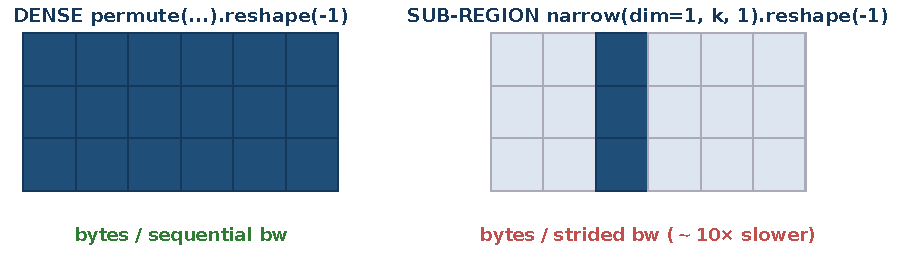
\includegraphics[width=0.78\linewidth]{figures/contiguity.pdf}
\caption{Contiguity-sensitive implicit copies. The same Python
\texttt{...reshape(-1)} is free on a dense permuted source (left,
sequential bw) but pays an $O(\text{numel})$ strided copy on a
sub-region narrow source (right, $4\times$--$10\times$ slower).}
\label{fig:contiguity}
\end{figure}

\paragraph{Side-by-side code: baseline vs agent AllToAllV.}
The agent's deployed AllToAllV runtime collapses the baseline's
AG$+$transpose$+$RS chain (two collectives plus a strided
permute/reshape) into a single padded \texttt{all\_gather} with a
metadata-only slice (Figures \ref{fig:a2av-baseline},
\ref{fig:a2av-agent}).

\begin{figure}[!htbp]
\centering
\begin{BVerbatim}[fontsize=\footnotesize]
def baseline_alltoallv(x, send_counts):
    # AG + transpose + RS path (2 collectives)
    cap = max_send_count(send_counts)
    padded = pad_to_cap(x, cap)
    full = xm.all_gather(padded, dim=0)
    full = full.view(ws, ws, cap, D)
    full = full.transpose(0, 1).contiguous()
    y = xm.reduce_scatter(
        xm.REDUCE_SUM, full.view(-1, D),
        scale=1.0, scatter_dim=0,
        shard_count=ws)
    return unpad(y, recv_counts)
\end{BVerbatim}
\caption{Internal-AWS-optimized baseline AllToAllV:
\texttt{all\_gather} + strided \texttt{permute}/\texttt{contiguous}
+ \texttt{reduce\_scatter}.}
\label{fig:a2av-baseline}
\end{figure}

\begin{figure}[!htbp]
\centering
\begin{BVerbatim}[fontsize=\footnotesize]
def agent_alltoallv(x, send_counts):
    # Pack-and-gather: ONE collective, no strided ops.
    cap = max_send_count(send_counts)
    packed = pack_to_dense(x, cap)
    gathered = xm.all_gather(packed, dim=0)
    gathered = gathered.view(ws, ws, cap, D)
    # Incoming slice is contiguous at outer-axis row `rank`:
    # metadata-only view + slice, no permute, no rs.
    return gathered[:, rank].reshape(-1, D)
\end{BVerbatim}
\caption{Agent-emitted AllToAllV (\emph{pack-and-gather}): one
collective, dispatch count halved, no strided
\texttt{permute}/\texttt{contiguous}. The metadata-only
\texttt{view+slice} replaces the chain that costs strided HBM
bandwidth in the baseline.}
\label{fig:a2av-agent}
\end{figure}



\section{Cost-model implementation details}
\label{sec:cost-impl}

This appendix collects the implementation-level details factored
out of §\ref{sec:cost} so the main text can stay at the
formula-and-idea level.

\subsection{Per-op floors and TrackedTensor recording}
\label{sec:cost-impl-local}

Pure-metadata view ops --- \texttt{view}, \texttt{narrow},
\texttt{transpose}, \texttt{permute}, \texttt{expand},
\texttt{squeeze}, \texttt{unsqueeze}, \texttt{flatten},
\texttt{slice} --- pay exactly the per-op floor; charging their
isolated-microbench cost (dominated by \texttt{mark\_step}
overhead) would penalize slice-loop chains that XLA actually fuses
inside one graph. The
\texttt{\_FUSED\_ELEMENTWISE\_OPS} category
floor-prices \texttt{mul}/\texttt{add}/\texttt{sub}/\texttt{div}/\texttt{mod}/\texttt{neg}
because adjacent elementwise ops fuse into one HLO kernel.
\texttt{TrackedTensor} overrides Python arithmetic dunders to
record into the same op counter the named-function calls use;
without this an algorithm that interleaves \texttt{*\,inv} between
\texttt{xm.all\_reduce} calls becomes event-stream-indistinguishable
from one that does not, and the back-to-back amortization in
§\ref{sec:cost-impl-coll} cannot disambiguate the two. The bytes
$b$ in every bytes-aware rule come from the actual PyTorch tensor
at trace time, not from declared shape.

\subsection{Four-tier amortization fitting}
\label{sec:cost-impl-coll}

The $\alpha_i$ coefficients are fit at Phase~1.
\texttt{measure\_back\_to\_back\_amortization}
returns total wall-clock time for $N$ back-to-back
\texttt{xm.all\_reduce} calls in one \texttt{mark\_step} graph at
configurable depth. When the LLM has probed at least depths
$\{1, 2, 4, 8\}$, the framework auto-fits each $\alpha_i$ as the
marginal per-issue cost in tier $i$ divided by the depth-1 (full)
cost. On a 7-node trn1.32xlarge cluster co-located in a single VPC
(AWS's per-account network isolation boundary, which the EFA
fabric requires because EFA peers must share an L2 broadcast
domain), the fit reliably converges to
$(\alpha_1, \alpha_2, \alpha_3) \approx (0.30, 0.10, 0.02)$ and
would re-fit if the EFA pipeline depth changes. The back-to-back
run resets on any non-free-XLA-op (which is why the
arithmetic-dunder recording from §\ref{sec:cost-impl-local} is
load-bearing).

\subsection{Launch and NEFF-reload constants}
\label{sec:cost-impl-launch}

The factor 2 in $T_{\text{launch}} = 2\,\ell\,m$ covers the
forward \texttt{mark\_step} and the implicit backward
\texttt{mark\_step} PyTorch/XLA inserts before
\texttt{loss.backward()} returns. The simulator AST-derives an
outer-loop graph-launch tax that contributes to $m$: each outer
\texttt{for m in range(M)} / \texttt{range(N\_MB)} /
\texttt{range(num\_microbatches)} loop (or any outer loop
containing an explicit \texttt{xm.mark\_step()}) charges
$2 \times \texttt{per\_graph\_neff\_load\_us}$ (default
$200\,\mu$s, doubled for fwd$+$bwd). Inner per-tensor / per-bucket
loops (\texttt{for g in rep\_grads}, \texttt{for bk in buckets})
do not pay this tax: at training scale the candidate function is
called once per step and those inner ops fuse into a single
back-to-back NEFF chain.

\subsection{Structural terms: fusion-credit, HBM safety,
primitive-viability}
\label{sec:cost-impl-struct}

Fusion-credit discount factor is set per cluster by the same
Phase-1 calibration that fits $\alpha_i$; on our cluster the
constant is $0.30$, fit against bundled-vs-per-microbatch HW
measurements across the three Llama-side model-extension
primitives in §\ref{sec:eval-llama}.

HBM safety uses default budget $2$\,GB/core, scale $10{,}000\,\mu$s.
The AST recognizes hardcoded byte-budget assignments
(\texttt{bucket\_bytes = 32 << 20}, \texttt{chunk\_bytes},
\texttt{partition\_bytes}, and their uppercase /
\texttt{max\_*\_bytes} / \texttt{*\_byte\_limit} /
\texttt{*\_cap\_bytes} variants) and clamps the simulated peak by
this cap before evaluating the quadratic penalty. The same cap
propagates to the \texttt{scaled\_bytes} of
\texttt{cat}/\texttt{stack}/\texttt{reshape}/\texttt{contiguous}
ops and to the \texttt{scaled\_max\_bytes} input of
$C(b_{\max})$; this prevents a bucketed algorithm from being
charged for a $\sim$30\,GB scaled tensor it never actually
materializes. The compilation-cost extrapolation $\hat C(b)$ also
uses the clamped value to avoid log-linear blowup past the largest
calibration sample.

Primitive-viability terms encode two real HW failure modes:
\texttt{xm.collective\_permute} ring patterns at world size $>64$
trigger a documented Trainium compiler SIGABRT; an
\texttt{xm.all\_reduce} payload past the Neuron Runtime's
per-collective tensor-size limit fails at
\texttt{LoadCollectives}. Both receive $+\infty$ cost.

\subsection{Phase-5 gate fallback and rationale}
\label{sec:cost-impl-phase5}

The HW microbench runs 20 iterations of the isolated candidate
call under \texttt{xla.step()} (this boundary forces a fresh
\texttt{mark\_step} graph per iteration, reporting steady-state
cost rather than a once-amortized compile). The training-validation
harness runs a 10-step bf16 training pass on an 8-layer DIM=1024
synthetic LM, bf16-only because that is Trainium's native
execution precision. When no Phase-3 candidate clears both gates
(e.g., every mutation tried to use a cluster-broken primitive at
training scale), Phase~5 falls back to the lowest-simulator-score
\emph{baseline} template --- a human-written seed known to compile
and run on this hardware --- rather than deploying a sim-only
winner that cannot load. This fallback was never triggered on the
eight problems evaluated; it is a robustness safety rail.


\section{Profiling tool details}
\label{sec:profile-impl}

The five $\Theta$ buckets are populated by seven
calibration tools the agent invokes through Phase~1's
\texttt{ToolBox}:
\begin{itemize}
  \item \texttt{measure\_algorithm\_latency} ---
  parameterized over primitive choice and tensor size for
  \texttt{all\_gather}, \texttt{reduce\_scatter},
  \texttt{all\_reduce}, \texttt{collective\_permute},
  \texttt{all\_to\_all}. Probes world sizes $\in \{4, 32, 224\}$
  and payload sizes $\in \{2^k : k = 10, \ldots, 22\}$ bytes,
  fits $T(b,N) = \alpha(N) + \beta(N) b$ per collective.
  \item \texttt{measure\_p2p\_transfer} --- disambiguates
  intra-node NeuronLink from inter-node EFA bandwidth.
  \item \texttt{measure\_xla\_op\_overhead} --- per-local-op
  floor.
  \item \texttt{measure\_compilation\_cost} --- fits the
  per-NEFF reload curve $C(b)$ over the largest collective tensor
  size (sweep $b \in \{2^{12}, 2^{16}, 2^{20}, 2^{24}\}$).
  \item \texttt{measure\_graph\_launch\_overhead} --- $\ell$, the
  per-\texttt{mark\_step} framework cost, measured as the
  marginal cost of $k+1$ no-op collectives in a single graph.
  \item \texttt{measure\_memory\_copy\_throughput} --- sequential
  and strided HBM bandwidth.
  \item \texttt{check\_cross\_node\_support} and
  \texttt{check\_primitive\_compilation} --- guardrails (catch
  cluster-broken primitives at calibration time, not at deployment).
\end{itemize}
The LLM picks call sites, sweeps, and aggregation strategy
autonomously --- it draws on its general knowledge of LLM
training, GPU and Trainium collective semantics, and
performance-engineering practice --- and produces the numerical
constants that populate the simulator. We supply the tools (so
the LLM cannot fabricate numbers), not the experimental design
(so the LLM exploits domain knowledge to choose probes more
informative than a hardcoded script would).


\section{Search-style prompt scaffolds}
\label{sec:search-prompts}

The three Phase-3 search styles share the Phase-1 simulator and
the Phase-4/5 gates but differ in how the LLM-time budget
$B = 1 + K + 2R$ calls is spent. The three figures below show the
system-prompt shape each style uses (paraphrased to one-page form;
the full templates live in \texttt{experiments/run\_search.py}).

\begin{figure}[!htbp]
\centering
\begin{BVerbatim}[fontsize=\footnotesize]
[SYSTEM]
You are designing a Trainium collective strategy.
Stage 1 (1 call): emit K=5 structurally distinct
  strategy sketches as (name, description) pairs.
Stage 2 (K=5 calls): implement each sketch as
  runnable Python; sandbox-validated at ws in {4,8}.
Stage 3 (2*R=4 calls): refine top-2 by Sim score.
  Each refine round: identify dominant cost term tau*
  in {T_local, T_coll, T_launch, T_NEFF, T_net};
  emit mutation s' that reduces tau*(s).
[USER]
Problem sig: <signature>
Seed templates: <S_P with Sim scores>
Theta (cost-model params): <flattened Phase-1 table>
\end{BVerbatim}
\caption{Strategy-enumerate prompt scaffold (default).}
\label{fig:prompt-strat}
\end{figure}

\begin{figure}[!htbp]
\centering
\begin{BVerbatim}[fontsize=\footnotesize]
[SYSTEM]
You are a Trainium collective-strategy refiner.
Run for 2*R*K = 20 ReAct turns. Each turn:
  Thought: analyze current strategy's bottleneck.
  Action: emit mutation s'.
  Observation: simulator returns Sim(s') and a
    per-term breakdown.
Keep the lowest-Sim strategy.
[USER]
Problem sig: <signature>; seed: <s_0>
Theta: <flattened>
\end{BVerbatim}
\caption{CC-ReAct prompt scaffold (single-trajectory).}
\label{fig:prompt-ccreact}
\end{figure}

\begin{figure}[!htbp]
\centering
\begin{BVerbatim}[fontsize=\footnotesize]
[SYSTEM]
You are a parallel mutation operator. K=5 islands
each hold one strategy. For r in 1..R rounds:
  for each island i:
    propose s'_i = M(s_i)  # LLM call
    if Sim(s'_i) < Sim(s_i): s_i <- s'_i
  every R/2 rounds, swap best of two random islands.
Total: K*R = 20 calls.
[USER]
Seeds: <K samples drawn from S_P>
Theta: <flattened>
\end{BVerbatim}
\caption{Multi-island GA prompt scaffold.}
\label{fig:prompt-mi}
\end{figure}


\section{Per-phase code snippets}
\label{sec:phase-code}

Each of the five phases corresponds to a compact entry point in
the codebase. The five figures below show the call shapes; the
full implementations live in \texttt{search/run\_search.py}.

\begin{figure}[!htbp]
\centering
\begin{BVerbatim}[fontsize=\footnotesize]
toolbox = build_calibration_tools(
    hw=trainium_7node)
Theta = M.calibrate(toolbox, max_calls=12)
# Theta = (Theta_net, Theta_launch, Theta_NEFF,
#         Theta_copy, Theta_neff_cache)
Sim = BuildCost(Theta)
\end{BVerbatim}
\caption{Phase 1 --- calibration.}
\label{fig:phase1}
\end{figure}

\begin{figure}[!htbp]
\centering
\begin{BVerbatim}[fontsize=\footnotesize]
pool = []
for s in S_P:
    if Verify(s, ref, ws={4,8}):
        pool.append((s, Sim(s)))
pool.sort(key=lambda x: x[1])  # by Sim
\end{BVerbatim}
\caption{Phase 2 --- baseline evaluation.}
\label{fig:phase2}
\end{figure}

\begin{figure}[!htbp]
\centering
\begin{BVerbatim}[fontsize=\footnotesize]
C = InitPool(S_P, sigma)
# sigma in {strat-enum, cc-react, multi-island}
for r in range(R):
    s_prime = M.propose(C, Theta)
    if not Verify(s_prime, ref): continue
    score = Sim(s_prime)
    C.add(s_prime, score,
          sigma_specific=True)
\end{BVerbatim}
\caption{Phase 3 --- LLM-driven search.}
\label{fig:phase3}
\end{figure}

\begin{figure}[!htbp]
\centering
\begin{BVerbatim}[fontsize=\footnotesize]
for s in C.survivors():
    t_hw = Microbench(s, hw, iters=20)
    shape_ok = ShapeGate(s, hw)
    tv_ok = TVGate(s, hw)
    if not (shape_ok and tv_ok):
        s = M.recover(s)  # up to 2 attempts
\end{BVerbatim}
\caption{Phase 4 --- hardware validation.}
\label{fig:phase4}
\end{figure}

\begin{figure}[!htbp]
\centering
\begin{BVerbatim}[fontsize=\footnotesize]
s_star = min(survived, key=Sim)
emit(f"runtime/trainium_{P.name}.py",
     s_star)
deploy_to(hw)
\end{BVerbatim}
\caption{Phase 5 --- code generation.}
\label{fig:phase5}
\end{figure}



\end{document}
